\documentclass[english,12pt,jmp,graphicx]{revtex4-1}
%\documentclass[jmp,graphicx]{revtex4-1}
%\documentclass[aip,reprint]{revtex4-1}

\usepackage{graphicx}% Include figure files
\usepackage{dcolumn}% Align table columns on decimal point
\usepackage{bm}% bold math
\usepackage{amsmath,amssymb,latexsym,mathrsfs}

\draft % marks overfull lines with a black rule on the right

\newtheorem{lemma}{Lemma}[section]
\newtheorem{theorem}{Theorem}[section]
\newtheorem{definition}{Definition}[section]
\newtheorem{remark}{Remark}[section]
\newtheorem{corollary}{Corollary}[section]


\newcommand{\ph}{\hat{\phi}}
\newcommand{\pt}{\tilde{\phi}}
\newcommand{\pc}{\check{\phi}}
\newcommand{\gh}{\hat{\gamma}}
\newcommand{\Dh}{\hat{\Delta}}
\newcommand{\dha}{\hat{\delta}}
\newcommand{\qh}{\hat{q}}
\newcommand{\xh}{\hat{x}}
\newcommand{\HM}{\mathcal{H}_{\text{max}}}
\newcommand{\Hm}{\mathcal{H}_{\text{min}}}
\newcommand{\sech}{\rm \hspace{0.7mm}sech}
\newcommand{\I}{\mathrm{i}}
\newcommand{\hh}{\hat{h}}
\newcommand{\mh}{m_r}
\newcommand{\mt}{m_i}

\begin{document}

% Use the \preprint command to place your local institutional report number 
% on the title page in preprint mode.
% Multiple \preprint commands are allowed.
%\preprint{}

\title{The Ising Model and a General Theory of Critical Transport
  Transitions in Binary Composite Media} %Title of paper

% repeat the \author .. \affiliation  etc. as needed
% \email, \thanks, \homepage, \altaffiliation all apply to the current author.
% Explanatory text should go in the []'s, 
% actual e-mail address or url should go in the {}'s for \email and \homepage.
% Please use the appropriate macro for the type of information

% \affiliation command applies to all authors since the last \affiliation command. 
% The \affiliation command should follow the other information.

\author{N. B. Murphy$^1$}
%\email[]{benmurphy.math@gmail.com}
%\homepage[]{Your web page}
%\thanks{}
%\altaffiliation{}
\affiliation{$(1)$ University of Utah, Department of Mathematics, 155 S 1400
  E RM 233, Salt Lake City, UT 84112-009, USA}
%
\collaboration{K. M. Golden$^1$}
%\author{K. M. Golden$^1$}
%\email[]{benmurphy.math@gmail.com}
%\homepage[]{Your web page}
%\thanks{}
%\altaffiliation{}
\affiliation{University of Utah, Department of Mathematics, 155 S 1400
  E RM 233, Salt Lake City, UT 84112-009, USA}

% Collaboration name, if desired (requires use of superscriptaddress option in \documentclass). 
% \noaffiliation is required (may also be used with the \author command).
%\collaboration{}
%\noaffiliation

\date{\today}

\begin{abstract}
%
We present a general critical theory for transport in binary
composite media holding for lattice and continuum percolation
models in the static, and frequency dependent (complex parameter) quasi--static
regimes. Through a direct, analytic correspondence between the 
magnetization of the Ising model and the effective parameter problem
of two--phase random media, we show that the critical exponents of
transport satisfy the standard scaling reations for phase transitions
in statistical mechanics. Analogus to the Lee--Yang--Ruelle
characterization of criticality in the Ising model, criticality in
transport is characterized by the collapse of spectral gaps and the
formation of delta function components in the underlying spectral measures.    
%
\end{abstract}

%\pacs{}% insert suggested PACS numbers in braces on next line

\maketitle %\maketitle must follow title, authors, abstract and \pacs

% Body of paper goes here. Use proper sectioning commands. 
% References should be done using the \cite, \ref, and \label commands
%
%------------------------------------------------------------------------
\section{Introduction}\label{sec:Introduction}
%
Lattice and continuum percolation models have been used to study a
broad range of disordered composite materials including semiconductors 
\cite{Efros-84}, radar absorbing coatings \cite{Kusy:N-58},
%thin films \cite{Davis:OC-70},
bone \cite{Sasaki:JTB:25,Golden:JoB:337}, rocks
\cite{Bourbie:JGR-11524,Broadbent:PCPS-629}, 
glacial ice \cite{Enting:1985:LSM}, polycrystalline metals
\cite{Chen:PRL:2007}, carbon nanotube composites
\cite{Kyrylyuk:PNAS:2008}, and sea ice \cite{Golden:S-2238}. A key
feature of these materials is the critical dependence of the effective
transport properties on the connectedness, or percolation properties,
of a particular component. The behavior of such composite media is
particularly challenging to describe physically, and to predict
mathematically.  

Here, we construct a mathematical framework which unifies the critical
theory of transport in two--phase random composite media. We accomplish this
by adapting techniques developed by G. A. Baker for the Ising model
\cite{Baker-1990}, to provide a detailed description of
percolation--driven critical transitions in transport exhibited by
such media. The most natural formulation of this problem is in terms
of the conduction problem in the continuum $\mathbb{R}^d$, which
includes the lattice $\mathbb{Z}^d$ as a special case
\cite{Golden:JMP-5627,Golden:CMP-473}. Although, the underlying
symmetries \cite{MILTON:2002:TC} in the effective parameter problem of
electrical conductivity and permittivity, magnetic permeability, and
thermal conductivity, generalize our results to all of these systems.     
%------------------------------------------------------------------------
\section{Background and Summary of our Results}\label{sec:Background}
%
In 1952 T. D. Lee and C. N. Yang showed that the root distribution of
the Ising model partition function $Z$, a polynomial in the activity
variable \cite{Lee:PR:411,Baker-1990,Ruelle-1969,Ruelle:AM:589},
completely determines the associated equation of state
\cite{Yang:PR:404}. Moreover, they demonstrated that the properties of 
the system, in relation to phase transitions, are governed by the
behavior of these roots near the positive real axis. They did so by
proving that the roots of $Z$ lie on the unit circle. This result is
known as the Lee--Yang Theorem \cite{Lee:PR:411,Ruelle-1969}.   

In 1968 G. A. Baker used the Lee--Yang Theorem to represent the Gibbs
free energy per spin $f=-(N\beta)^{-1}\ln{Z}$ as a logarithmic potential
\cite{Saff_Totik:97}, where $N$ is the number of spins, $\beta=(kT)^{-1}$,
$k$ is Boltzmann's constant, and $T$ is the absolute temperature
\cite{Baker:PRL-990}. He used this special analytic structure to prove
that the magnetization per spin $M(T,H)=-\partial f/\partial H$
\cite{Robertson-1993} may be represented in terms of a Stieltjes
function $G$ in the variable $\tau=\tanh{\beta mH}$,          
%
\begin{align}\label{Ising_Stieltjes_Fun}
  \frac{M}{m} =\tau(1+(1-\tau^2)G(\tau^2)), \quad
  G(\tau^2)=\int_0^\infty\frac{d\psi(y)}{1+\tau^2y}\,, % for single column paper
  %\frac{M(T,H)}{m} =\tau(1+(1-\tau^2)G(\tau^2)), \\
  %G(\tau^2)=\int_0^\infty\frac{d\psi(y)}{1+\tau^2y}\;,\notag % for two column paper
\end{align}
%
where $H$ is the applied magnetic field strength, $m$ is the
(constant) magnetic dipole moment of each spin \cite{Griffiths-1999},
and $\psi$ is a non--negative definite measure \cite{Baker:PRL-990,Baker-1990}. The
integral representation \eqref{Ising_Stieltjes_Fun} immediately leads
to the inequalities    
%
\begin{align}\label{eq:Gtau_inneq}
  G\geq0, \qquad \frac{\partial G}{\partial u}\leq0, \qquad \frac{\partial^2G}{\partial u^2}\geq0,
\end{align}
%
where $u=\tau^2$. The last formula in equation \eqref{eq:Gtau_inneq} is
the GHS inequality, which is an important tool in the study of the
Ising model \cite{Golden:JMP-5627}. 

In 1970 D. Ruelle extended the Lee--Yang Theorem and proved that
there exists a gap $\theta_0(T)>0$ in the roots of $Z$ about the positive
real axis for high temperatures \cite{Ruelle:PRL:303}. Moreover, he
proved that the gap collapses $(\theta_0(T)\to0)$ as $T$ decreases to a
critical temperature $T_c>0$. Consequently, the temperature--driven
phase transition (spontaneous magnetization) is unique, and is
characterized by the pinching of the real axis by the roots of $Z$
\cite{Ruelle-1969}.   

In \cite{Baker:PRB:1184,Baker-1990} G. A. Baker exploited the
Lee--Yang--Ruelle Theorem and provided a detailed description of the 
percolation aspects of the phase transition
\cite{Christensen-2005}. He defined a critical 
exponent $\Delta$ for the gap in the distribution of the Lee--Yang--Ruelle
zeros, $\theta_0(T)\sim(T-T_c)^\Delta$, as $T\to T_c^+$, and proved that
%the support $\Sigma_\psi$ of
the measure $\psi$ is supported on the compact interval
$[0,S(T)]$ for $T>T_c\,$, with $S(T)\sim(T-T_c)^{-2\Delta}$ as
$T\to T_c^+$. He demonstrated that the moments $\psi_n=\int_0^\infty y^n\,d\psi(y)$
%of $\psi$
diverge as $T\to T_c^+$ according to the
power law $\psi_n\sim(T-T_c)^{-\gamma_n}$, $n\geq0$. 
%Using a Stieltjes function characterization theorem \cite{Baker-1990},
He showed that the sequence $\gamma_n$ satisfies Baker's inequalities
$\gamma_{n+1}-2\gamma_n+\gamma_{n-1}\geq0$, which imply that this sequence increases at
least linearly with $n$, and that this sequence is actually
linear in $n$, $\gamma_n=\gamma+2\Delta n$, with constant gap $\gamma_i-\gamma_{i-1}=2\Delta$
\cite{Baker-1990}. The critical exponent $\gamma$ is defined via the 
magnetic susceptibility per spin $\chi=\partial M/\partial H=-\partial^2f/\partial H^2\sim(T-T_c)^{-\gamma}$, as
$T\to T_c^+$. The phase transition may be concisely described with two
other critical exponents. When $H=0$, $M(T,0)\sim(T-T_c)^\beta$, as $T\to T_c^-$,
where the critical exponent $\beta$ is not to be confused with
$(kT)^{-1}$, and along the critical isotherm $T=T_c$, $M(T_c,H)\sim H^{1/\delta}$,
as $H\to0$ \cite{Christensen-2005,Baker-1990}. Using the integral
representation \eqref{Ising_Stieltjes_Fun}, Baker obtained 
(two--parameter) scaling relations between the critical exponents
\cite{Baker-1990} 
%
\begin{align}\label{eq:Ising_Scaling_Relations}
  \beta=\Delta-\gamma, \qquad \delta=\Delta/(\Delta-\gamma), \qquad \gamma_n=\gamma+2\Delta n.
\end{align}
%
The critical exponent $\gamma$, for example, is defined
in terms of the following limit, and $\gamma$ exists when this limit exists
\cite{Baker-1990}:
% 
\begin{align}\label{eq:Critical_Exponent_Existence}
  \gamma:=\limsup_{T\to T_c^+, \;H=0}\left(\frac{-\ln \chi(T,H)}{\ln(T-T_c)}  \right).
\end{align}
%

In 1997 K. M. Golden demonstrated that Baker's critical theory may be
adapted to precisely describe percolation--driven critical transitions
in transport, exhibited by two--phase random media in the static regime
\cite{Golden:PRL-3935}. This deep and far reaching result puts these 
two classes of seemingly unrelated problems on an equal mathematical
footing. He did so by considering percolation models of classical
conductive binary composite media, where the connectedness of the
system is determined by the volume fraction $p$ of defect inclusions
with conductance $\sigma_2$ in an otherwise homogeneous medium of
conductance $\sigma_1$, and by assumption $h=\sigma_1/\sigma_2\in[0,1)$.
He demonstrated that the function $m(p,h)=\sigma^*(p,h)/\sigma_2$ plays the role of
the magnetization  $M(T,H)$ in the Ising model, where
$\sigma^*$ is the effective conductance of the
%random
medium \cite{Bergman:PRC-377,Milton:APL-300,Golden:CMP-473}. Moreover, he
showed that the volume fraction $p$ mimics the temperature $T$ while
the contrast ratio $h$ mimics the applied magnetic field strength $H$. More
specifically, critical insulator/conductor behavior in transport
arises when $h=0$ $(\sigma_1=0, \ 0<\sigma_2<\infty)$, as $p\to p_c^+$
\cite{Golden:PRL-3935}, and non-magnetic/ferromagnetic
critical behavior of the Ising model arises when $H=0$, as $T\to T_c^+$
\cite{Christensen-2005}. Using these mathematical
parallels, Golden showed that the critical exponents of transport
satisfy an analogue of Baker's %two--parameter
scaling relations \eqref{eq:Ising_Scaling_Relations}.

Here, using a novel unified approach, we reproduce Golden's
static results $(h\in\mathbb{R})$ and produce the analogous
static results associated with a conductive--superconductive medium in
terms of $w(p,z)=\sigma^*(p,z)/\sigma_1$, where $z=1/h$. Using Stieltjes
function integral representations of $m(p,h;\mu)$ and $w(p,z;\alpha)$, where
$\mu$ and $\alpha$ are each spectral measures of a self--adjoint random operator, we
determine the (two--parameter) critical exponent scaling relations of each
system. We then extend these results to the frequency dependent
quasi-static regime $(h\in\mathbb{C})$. We link these two sets of
critical exponents, showing that they are all, in general, determined
by only three critical exponents, and are determined by only two
critical exponents under a physically consistent symmetry in the
properties of $\mu$ and $\alpha$. In arbitrary, finite lattice systems we
explicitly show that there are gaps in the supports of the measures
$\alpha(d\lambda)$ and $\mu(d\lambda)$ about the spectral endpoints $\lambda=0,1$ for $p\ll1$ and
$1-p\ll1$, respectively, which collapse as $p$ tends towards
$p_c$. Moreover in infinite lattice, or continuum composite systems, we demonstrate that
critical transitions in transport are due to the formation of delta
function components in $\mu$ and $\alpha$ located at $\lambda=0,1$. We do so by
constructing a measure $\varrho(d\lambda)$ that is supported on the set $\{0,1\}$
which links the measures $\mu$ and $\alpha$. This general result demonstrates
that, for percolation models, the onset of criticality (the formation
of these delta components) occurs \emph{precisely} at the percolation
threshold $p_c$.  
%
%------------------------------------------------------------------------------
%
\section{The Analytic Continuation Method}\label{eq:TACM}
%
We now formulate the effective parameter problem for two--component
conductive media. Let $(\Omega,P)$ be a probability space, and let
$\bm{\sigma}(\vec{x},\omega)$ and $[\bm{\sigma}^{-1}](\vec{x},\omega)$ be the local
conductivity and resistivity tensors, respectively, which are
(spatially) stationary random fields in $\vec{x}\in\mathbb{R}^d$ and
$\omega\in\Omega$. Here $\Omega$ is the set of all geometric realizations of our random medium
and $P(d\omega)$ is the underlying probability measure, which is compatible
with stationarity \cite{Golden:CMP-473}. Define the Hilbert space of
stationary random fields $\mathscr{H}_s\subset L^2(\Omega,P)$, and the underlying
Hilbert spaces of stationary curl free $\mathscr{H}_\times\subset\mathscr{H}_s$
and divergence free $\mathscr{H}_{\bullet}\subset\mathscr{H}_s$ random fields
\cite{Golden:CMP-473} 
%
\begin{align}\label{eq:curlfreeHilbert}
  &\mathscr{H}_\times:=
  \{\vec{Y}(\omega)\in \mathscr{H}_s \ | \ \vec{\nabla} \times\vec{Y}=0 \text{ weakly and }
    \langle\vec{Y}\rangle=0\}, \\
&\mathscr{H}_{\bullet}:=
\{\vec{Y}(\omega)\in \mathscr{H}_s \ | \ \vec{\nabla}\cdot\vec{Y}=0 \text{ weakly and }
    \langle\vec{Y}\rangle=0\},\notag
\end{align}
%
where $\vec{Y}:\Omega\mapsto\mathbb{R}^d$ and $\langle\cdot\rangle$ means ensemble average over
$\Omega$, or by an ergodic theorem \cite{Golden:CMP-473} spatial average
over all of ${\mathbb{R}}^d$. 

Consider the following variational problems: 
find $\vec{E}_f\in\mathscr{H}_\times$ and  $\vec{J}_f\in \mathscr{H}_{\bullet}$ such
that    
%
\begin{align}
  \label{eq:Weak_Curl_Free_Variational_Form}
 &\langle\bm{\sigma}(\vec{E}_0+\vec{E}_f)\cdot\vec{Y}\rangle=0 \quad  \forall \
  \vec{Y}\in\mathscr{H}_\times &&\text{and}
%
 &&\langle\bm{\sigma}^{-1}(\vec{J}_0+\vec{J}_f)\cdot\vec{Y}\rangle=0 \quad  \forall \
  \vec{Y}\in\mathscr{H}_{\bullet}\,,  
\end{align}
%
respectively \cite{Golden:CMP-473}. Under the assumption that the
bilinear forms
$a(\vec{u},\vec{v})=\vec{u}^{\,T}\bm{\sigma}(\vec{x},\omega)\vec{v}$ and
$\tilde{a}(\vec{u},\vec{v})=\vec{u}^{\,T}[\bm{\sigma}^{-1}](\vec{x},\omega)\vec{v}$
are bounded and coercive, where $\vec{u},\vec{v}\in\mathbb{R}^d$, these
problems have unique solutions satisfying \cite{Golden:CMP-473} 
%
\begin{align}   \label{eq:Maxwells_Equations_E}  
  &\vec{\nabla}\times\vec{E}=0, &&
  \vec{\nabla}\cdot\vec{J}=0,&&
  \vec{J}=\bm{\sigma}\vec{E},&&
  \vec{E}=\vec{E}_0+\vec{E}_f, &&
  \langle\vec{E}\,\rangle=\vec{E}_0, \\
%
  %\label{eq:Maxwells_Equations_D}
   &\vec{\nabla}\times\vec{E}=0, &&
   \vec{\nabla}\cdot\vec{J}=0, &&
   \vec{E}=\bm{\sigma}^{-1}\vec{J},&&
   \vec{J}=\vec{J}_0+\vec{J}_f,&&
   \langle\vec{J}\,\rangle=\vec{J}_0,\notag
\end{align}
%
respectively. Here $\vec{E}_f$ and $\vec{J}_f$ are the fluctuating
electric field and current density of mean zero, respectively, about the
(constant) averages $\vec{E}_0$ and $\vec{J}_0$, respectively. 

We assume that the tensor $\bm{\sigma}(\vec{x},\omega)$ takes the values $\sigma_1$
and $\sigma_2$, and that the tensor $[\bm{\sigma}^{-1}](\vec{x},\omega)$ takes the
values $1/\sigma_1$ and $1/\sigma_2$, and write 
$\bm{\sigma}(\vec{x},\omega):=\sigma_1\chi_1(\vec{x},\omega)+\sigma_2\chi_2(\vec{x},\omega)$ and
$[\bm{\sigma}^{-1}](\vec{x},\omega):=\chi_1(\vec{x},\omega)/\sigma_1+\chi_2(\vec{x},\omega)/\sigma_2$.
Here, $\chi_j$ is the characteristic function of medium $j=1,2$, which
equals one for all $\omega\in\Omega$ having medium $j$ at $\vec{x}$, and zero
otherwise \cite{Golden:CMP-473}. As $\vec{E}_f\in\mathscr{H}_\times$ and
$\vec{J}_f\in\mathscr{H}_{\bullet}$, equation
\eqref{eq:Weak_Curl_Free_Variational_Form}
yields the energy (power density) constraints
$\langle\vec{J}\cdot\vec{E}_f\rangle=\langle\vec{E}\cdot\vec{J}_f\rangle=0$, which lead to the
reduced energy representations   
%
\begin{align}\label{eq:Reduced_System_Energy_Representations}
  \langle\vec{J}\cdot\vec{E}\rangle=\langle\vec{J}\rangle\cdot\vec{E}_0 \quad \text{and} \quad
  \langle\vec{E}\cdot\vec{J}\rangle=\langle\vec{E}\rangle\cdot\vec{J}_0\,.
\end{align}
%
%In light of \eqref{eq:Reduced_System_Energy_Representations}, we define
The effective complex conductivity and resistivity tensors, $\bm{\sigma}^*$
and $[\bm{\sigma}^{-1}]^*$, are defined by  
%
\begin{align}\label{eq:eff_eps_def}
    \langle \vec{J} \,\rangle=  \bm{\sigma}^* \vec{E}_0 \quad \text{and} \quad
    %\quad \text{and}  \quad 
    \langle \vec{E} \,\rangle=  [\bm{\sigma}^{-1}]^*\vec{J}_0,
\end{align}
%
respectively. For simplicity, we focus on one diagonal component of
these symmetric tensors: $\sigma^*:=\bm{\sigma}^*_{kk}$ and
$[\sigma^{-1}]^*:=[\bm{\sigma}^{-1}]^*_{kk}$, for some $k=1,\ldots,d$.

Due to the homogeneity of these functions, e.g.
$\sigma^*(a\sigma_1,a\sigma_2)=a\sigma^*(\sigma_1,\sigma_2)$ for any complex number $a$,
%$\sigma^*$ and $[\sigma^{-1}]^*$
they depend only on the ratio $h:=\sigma_1/\sigma_2$, and we define the
dimensionless functions $m(h):=\sigma^*/\sigma_2$, $w(z):=\sigma^*/\sigma_1$,
$\tilde{m}(h):=\sigma_1[\sigma^{-1}]^*$, and $\tilde{w}(z):=\sigma_2[\sigma^{-1}]^*$, where 
$z=z(h):=1/h$. The functions $m(h)$ and $\tilde{m}(h)$ are analytic off the
negative real axis in the $h$--plane, and the functions $w(z)$ and
$\tilde{w}(z)$ are analytic off the negative real axis in the
$z$--plane \cite{Golden:CMP-473}. Each take the corresponding upper
half plane to the upper half plane, so that they are examples of 
Herglotz functions \cite{Golden:CMP-473}. We assume that $0<|h|<1$,
i.e. $0<|\sigma_1|<|\sigma_2|<\infty$, and we further restrict $h$ the set
%
\begin{align}\label{eq:h_Domain}
  \mathcal{U}:=\{h\in\mathbb{C}: |h|<1 \text{ and } h\not\in(-1,0]\}.
\end{align}
%
%where $m$, $\tilde{m}$, $w$, and $\tilde{w}$ are analytic functions of
%$h$ \cite{Golden:CMP-473}.
In order to illuminate the symmetries between these functions, we will henceforth
focus on the complex variable $h:=h_r+\I h_i$, where
$h_r=\text{Re}(h)$ and $h_i=\text{Im}(h)$.

The key step in the method is obtaining integral representations for
$\sigma^*$ and $[\sigma^{-1}]^*$. These integral representations are given in
terms of resolvent representations of the electric field $\vec{E}$ and
the current density $\vec{J}$,   
%
\begin{align}\label{eq:Resolvent_representations_E_D}
  \vec{E}=s(s+\Gamma\chi_1)^{-1}\vec{E}_0=t(t+\Gamma\chi_2)^{-1}\vec{E}_0,\qquad
  \vec{J}=s(s-\Upsilon\chi_2)^{-1}\vec{J}_0=t(t-\Upsilon\chi_1)^{-1}\vec{J}_0,
\end{align}
%
where we have defined $s:=1/(1-h)$ and $t:=1/(1-z)=1-s$. These
formulas follow from manipulations of equation
\eqref{eq:Maxwells_Equations_E}. The operator 
$-\Gamma:=-\vec{\nabla}(-\Delta)^{-1}\vec{\nabla}\cdot$ is a projection onto curl-free fields,
based on convolution with the free-space Green's function for the
Laplacian $-\Delta=-\nabla^{\,2}$ \cite{Golden:CMP-473}. More specifically,
$-\Gamma:\mathscr{H}_s\mapsto\mathscr{H}_\times$ and for every
$\vec{\zeta}\in\mathscr{H}_\times$, we have $-\Gamma\vec{\zeta}=\vec{\zeta}$. To the authors  
knowledge, the operator $\Upsilon:=\vec{\nabla}\times(-\Delta)^{-1}\vec{\nabla}\times$ is being
introduced here for the first time. For the convenience of the reader,
we recall a few vector calculus facts. For every
$\vec{\zeta}\in\mathscr{H}_\bullet$ we have $\vec{\zeta}=\vec{\nabla}\times(\vec{A}+\vec{C})$
weakly, where $\vec{\nabla}\times\vec{C}=0$ weakly \cite{Jackson-1999}. The
arbitrary vector $\vec{C}$ can be chosen so that $\vec{\nabla}\cdot\vec{A}=0$
weakly \cite{Jackson-1999}. Hence,
$\vec{\nabla}\times\vec{\zeta}=\vec{\nabla}\times\vec{\nabla}\times\vec{A}
=\vec{\nabla}(\vec{\nabla}\cdot\vec{A})-\Delta\vec{A}=-\Delta\vec{A}$ weakly. The vector
$\vec{C}$ chosen in this manner gives the Coulomb (or transverse)
gauge of $\vec{\zeta}$ \cite{Jackson-1999}. Let
$\mathscr{C}_{\bullet}\subset\mathscr{H}_{\bullet}$ denote the \emph{closure} of the
space of stationary divergence free random fields of Coulomb gauge. On
the Hilbert space $\mathscr{C}_{\bullet}$, one can show that the
operator $\Upsilon$ is a projector, based on convolution with the
free-space Green's function for the Laplacian $-\Delta$. More specifically,
$\Upsilon:\mathscr{H}_s\mapsto\mathscr{H}_\bullet$ and for every $\vec{\zeta}\in\mathscr{C}_\bullet$,
we have $\Upsilon\vec{\zeta}=\vec{\zeta}$.  

It is more convenient to consider the functions
$F(s):=1-m(h)$ and $E(s):=1-\tilde{m}(h)$, which are
analytic off $[0,1]$ in the $s$--plane, and $G(t):=1-w(z(h))$ and
$H(t):=1-\tilde{w}(z(h))$, which are analytic off $[0,1]$ in the
$t$--plane \cite{Bergman:PRC-377,Golden:CMP-473}, and satisfy
%
\begin{align}\label{eq:Stieltjes_Bounds}
  0<|F(s)|,|E(s)|<1, \quad 0<|G(t)|,|H(t)|<\infty,\quad h\in\mathcal{U}
\end{align}
%
where $G(t)$ and $H(t)$ are not to be confused with the Stieltjes
function in \eqref{Ising_Stieltjes_Fun} and the magnetic field
strength in the Ising model, respectively. We write $\vec{E}_0=E_0\,\vec{e}_k$ and
$\vec{J}_0=J_0\,\vec{j}_k$, where $\vec{e}_k$ and $\vec{j}_k$ are unit
vectors, for some $k=1,\ldots,d$. 
%
% Using $\vec{J}=\sigma\vec{E}$,
% $\vec{E}=[\sigma^{-1}]\,\vec{J}$, $\langle\vec{E}\,\rangle=\vec{E}_0$,
% $\langle\vec{J}\,\rangle=\vec{J}_0$, and $\chi_1=1-\chi_2$ (which leads to the identities
% $\sigma=\sigma_2(1-\chi_1/s)=\sigma_1(1-\chi_2/t)$ and
% $[\sigma^{-1}]=(1-\chi_2/s)/\sigma_1=(1-\chi_1/t)/\sigma_2$),     
% %
% \begin{align}\label{eq:conductivity_identities}
%   &\sigma=\chi_1\sigma_1+\chi_2\sigma_2=\sigma_2(h\chi_1+\chi_2)=\sigma_2(1-\chi_1/s), \\
%   &\sigma=\chi_1\sigma_1+\chi_2\sigma_2=\sigma_1(\chi_1+z\chi_2)=\sigma_1(1-\chi_2/t),  \notag\\
%   &[\sigma^{-1}]=\chi_1/\sigma_1+\chi_2/\sigma_2=(\chi_1+h\chi_2)/\sigma_1=(1-\chi_2/s)/\sigma_1, \notag\\
%   &[\sigma^{-1}]=\chi_1/\sigma_1+\chi_2/\sigma_2=(z\chi_1+\chi_2)/\sigma_2=(1-\chi_1/t)/\sigma_2, \notag 
% \end{align}
% %
Using $\chi_1=1-\chi_2$ and equations \eqref{eq:Maxwells_Equations_E},
\eqref{eq:eff_eps_def}, and \eqref{eq:Resolvent_representations_E_D},
the Spectral Theorem \cite{Reed-1980} yields
\cite{Golden:CMP-473,Bergman:PRC-377}
% % 
% \begin{align}\label{eq:Herglotz_Funs_sed_LYRB}
%   F(s)&=\langle\chi_1(s+\Gamma\chi_1)^{-1}\vec{e}_k\cdot\vec{e}_k\rangle
%        =\int_{\lambda_0}^{\lambda_1}\frac{d\mu(\lambda)}{s-\lambda}\,,
%        \\
% %       
%   E(s)&=\langle\chi_2(s-\Upsilon\chi_2)^{-1}\vec{j}_k\cdot\vec{j}_k\rangle
%        =\int_{\tilde{\lambda}_0}^{\tilde{\lambda}_1}\frac{d\eta(\lambda)}{s-\lambda}\,,
%    \notag \\
% %   
%   G(t(s))&=\langle\chi_2(1-s+\Gamma\chi_2)^{-1}\vec{e}_k\cdot\vec{e}_k\rangle
%        =-\int_{1-\hat{\lambda}_1}^{1-\hat{\lambda}_0}\frac{[-d\alpha(1-\lambda)]}{s-\lambda}\,,
%    \notag \\
% %   
%   H(t(s))&=\langle\chi_1(1-s-\Upsilon\chi_1)^{-1}\vec{j}_k\cdot\vec{j}_k\rangle
%        =-\int_{1-\check{\lambda}_1}^{1-\check{\lambda}_0}\frac{[-d\kappa(1-\lambda)]}{s-\lambda}\,.
%   \notag
% \end{align}
% %
% 
\begin{align}\label{eq:Herglotz_Funs_sed_LYRB}
  &F(s)=\langle\chi_1(s+\Gamma\chi_1)^{-1}\vec{e}_k\cdot\vec{e}_k\rangle
       :=\int_{\lambda_0}^{\lambda_1}\frac{d\mu(\lambda)}{s-\lambda}\,,
       &&
%       
  E(s)=\langle\chi_2(s-\Upsilon\chi_2)^{-1}\vec{j}_k\cdot\vec{j}_k\rangle
       :=\int_{\tilde{\lambda}_0}^{\tilde{\lambda}_1}\frac{d\eta(\lambda)}{s-\lambda}\,,
    \\
%   
  &G(t)=\langle\chi_2(t+\Gamma\chi_2)^{-1}\vec{e}_k\cdot\vec{e}_k\rangle
       :=\int_{\hat{\lambda}_0}^{\hat{\lambda}_1}\frac{d\alpha(\lambda)}{t-\lambda}\,,
    &&
%   
  H(t)=\langle\chi_1(t-\Upsilon\chi_1)^{-1}\vec{j}_k\cdot\vec{j}_k\rangle
       :=\int_{\check{\lambda}_0}^{\check{\lambda}_1}\frac{d\kappa(\lambda)}{t-\lambda}\,.
  \notag
\end{align}
%
In order to illuminate the symmetries between the integral
representations of \eqref{eq:Herglotz_Funs_sed_LYRB}, in the last two
formulas of equation \eqref{eq:Herglotz_Funs_sed_LYRB} we will
henceforth make the change of variables $t(s)=1-s$ and
$\lambda\mapsto1-\lambda$, so that
$G(t(s))=-\int_{1-\hat{\lambda}_1}^{1-\hat{\lambda}_0}[-d\alpha(1-\lambda)]/(s-\lambda)$, for example.   

In equation \eqref{eq:Herglotz_Funs_sed_LYRB}, $\mu$, $\eta$, $\alpha$, and $\kappa$ 
are bounded positive measures which depend only on the geometry of the
medium. They are supported on $\Sigma_\mu,\Sigma_\eta,\Sigma_\alpha,\Sigma_\kappa\subseteq[0,1]$, respectively,
where the supremum and infimum of these sets are defined to be the
respective upper and lower limits of integration in
\eqref{eq:Herglotz_Funs_sed_LYRB} \cite{Golden:CMP-473,Bergman:AP-78}. 
%
% $\Sigma_\mu\subseteq[\lambda_0,\lambda_1]$, $\Sigma_\eta\subseteq[\tilde{\lambda}_0,\tilde{\lambda}_1]$,
% $\Sigma_\alpha\subseteq[\hat{\lambda}_0,\hat{\lambda}_1]$, and $\Sigma_\kappa\subseteq[\check{\lambda}_0,\check{\lambda}_1]$.
%
% $\lambda_0:=\inf(\Sigma_\mu)$, $\lambda_1:=\sup(\Sigma_\mu)$, $\tilde{\lambda}_0:=\inf(\Sigma_\eta)$,
% $\tilde{\lambda}_1:=\sup(\Sigma_\eta)$, $\hat{\lambda}_0:=\inf(\Sigma_\alpha)$,
% $\hat{\lambda}_1:=\sup(\Sigma_\alpha)$, $\check{\lambda}_0:=\inf(\Sigma_\kappa)$, and
% $\check{\lambda}_1:=\sup(\Sigma_\kappa)$.
%
The Integro-differential operators $\mathbf{M}_j:=\chi_j(-\Gamma)\chi_j$ and
$\mathbf{K}_j:=\chi_j\Upsilon\chi_j$, $j=1,2$, are compositions of projection
operators on the associated Hilbert spaces $\mathscr{H}_\times$ and
$\mathscr{C}_\bullet$, and are consequently bounded by 1 in the underlying
operator norm \cite{Rudin:87,Folland:95}. They are self--adjoint on
$L^2(\Omega,P)$ \cite{Golden:CMP-473}. Consequently, in the Hilbert space $L^2(\Omega,P)$
with weight $\chi_2$ in the inner product, for example, $\Gamma\chi_2$ is a 
bounded self--adjoint operator \cite{Golden:CMP-473}. Equation
\eqref{eq:Herglotz_Funs_sed_LYRB} involves spectral representations of
resolvents involving these self adjoint operators. The measures $\mu$,
$\eta$, $\alpha$, and $\kappa$ are spectral measures of the family of projections
of these operators in the respective $\langle\vec{e}_k,\vec{e}_k\rangle$ or
$\langle\vec{j}_k,\vec{j}_k\rangle$ state \cite{Golden:CMP-473,Reed-1980}.   

A key feature of equations
\eqref{eq:Reduced_System_Energy_Representations}--\eqref{eq:eff_eps_def} and
\eqref{eq:Herglotz_Funs_sed_LYRB} is 
that the parameter information in $s$ and $E_0$ is {\it separated}
from the geometry of the composite, which is encapsulated in the 
measures $\mu$, $\eta$, $\alpha$, and $\kappa$ through their moments $\mu_n$, $\eta_n$,
$\alpha_n$, and $\kappa_n$, $n\geq0$, which depend on the correlation functions of the
medium \cite{Golden:CMP-473}. For example, $\alpha_0=\eta_0=p$ and
$\mu_0=\kappa_0=1-p$. A principal application of the analytic continuation
method is to derive \emph{forward bounds} on $\sigma^*$ and $[\sigma^{-1}]^*$, given partial
information on the microgeometry
\cite{Bergman:PRL-1285,Milton:APL-300,Golden:CMP-473,Bergman:AP-78}. One
can also use the integral representations
\eqref{eq:Herglotz_Funs_sed_LYRB} to obtain \emph{inverse bounds},
allowing one to use data about the electromagnetic response of a
sample to bound its structural parameters such as $p$ \cite{Golden:JoB:337}.
%(\cite{Golden:JoB:337} and references therein). 

By applying the Spectral Theorem to the energy constraints
$\langle\vec{J}\cdot\vec{E}_f\rangle=\langle\vec{E}\cdot\vec{J}_f\rangle=0$, we have obtained detailed
decompositions of the system energy in terms of the measures $\mu$, $\eta$,
$\alpha$, and $\kappa$. For example, $\langle\vec{J}\cdot\vec{E}_f\rangle=0$,
$\vec{E}=\vec{E}_0+\vec{E}_f$, $\langle\vec{E}_f\,\rangle=0$, and
$\sigma=\sigma_2(1-\chi_1/s)$ imply that $0=\langle\sigma\vec{E}\cdot\vec{E}_f\rangle=\langle\sigma_2(1-\chi_1/s)(\vec{E}_f\cdot\vec{E}_0+E_f^2)\rangle
  =\sigma_2\left[\langle E_f^2\rangle- (\langle\chi_1\vec{E}_f\cdot\vec{E}_0\rangle
      + \langle\chi_1E_f^2\rangle)/s\right].$
% %
% \begin{align*}
%   0=\langle\sigma\vec{E}\cdot\vec{E}_f\rangle=\langle\sigma_2(1-\chi_1/s)(\vec{E}_0\cdot\vec{E}_f+E_f^2)\rangle
%  =\sigma_2\left(\langle E_f^2\rangle- \frac{1}{s}\left(\langle\chi_1\vec{E}_0\cdot\vec{E}_f\rangle
%      + \langle\chi_1E_f^2\rangle\right)\right).
% \end{align*}
% %
Therefore, by the Spectral Theorem \cite{Reed-1980} and the symmetries
in equation \eqref{eq:Herglotz_Funs_sed_LYRB} we have
%
\begin{align}\label{eq:Herglotz_energy_Reps}
 &\frac{\langle E_f^2\rangle}{E_0^2}=\int_0^1 \frac{\lambda\,d\mu(\lambda)}{(s-\lambda)^2}
           =\int_0^1 \frac{\lambda\,d\alpha(\lambda)}{(1-s-\lambda)^2}\,, 
 &&\frac{\langle J_f^2\rangle}{J_0^2}=\int_0^1 \frac{\lambda\,d\eta(\lambda)}{(s-\lambda)^2}
           =\int_0^1 \frac{\lambda\,d\kappa(\lambda)}{(1-s-\lambda)^2}\,.
\end{align}
%
Equation \eqref{eq:Herglotz_energy_Reps} then leads to Herglotz
function representations of all such energy components involving the
spectral measures $\mu$, $\eta$, $\alpha$, and $\kappa$,
e.g. $\langle\vec{E}\cdot\vec{E}_f\rangle/E_0^2=\int_0^1d\mu(\lambda)/(s-\lambda)^2$.%=\int_0^1d\alpha(\lambda)/(1-s-\lambda)^2$.

The Stieltjes transforms \eqref{eq:Herglotz_Funs_sed_LYRB} of the
measures $\mu$, $\eta$, $\alpha$, and $\kappa$ may be represented in terms of Stieltjes 
functions \cite{Baker-1990} of $h$ via the following change of variables:
$s(h)=1/(1-h)$ and $\lambda(y)=y/(1+y)\iff y(\lambda)=\lambda/(1-\lambda)$. For example,
%
\begin{align}\label{eq:var_subs_Fs}
  F(s)=%\int_{S_0}^{S}\frac{d\mu(\frac{y}{1+y})}
         %       {\frac{1}{1-h}-\frac{y}{1+y}}
                %:=
                (1-h)\int_{S_0}^{S}\frac{(1+y)d\mu(\frac{y}{1+y})}{1+hy}
                %:=(1-h)\int_{S_0}^{S}\frac{d\phi(y)}{1+hy}
                \,,  \qquad
  G(t(s))=%-\int_{\hat{S}_0}^{\hat{S}}\frac{[-d\alpha(\frac{1}{1+y})]}
           %     {\frac{1}{1-h}-\frac{y}{1+y}}
                %:=
                (h-1)\int_{\hat{S}_0}^{\hat{S}}\frac{(1+y)[-d\alpha(\frac{1}{1+y})]}{1+hy}
                %:=(h-1)\int_{\hat{S}_0}^{\hat{S}}\frac{d\ph(y)}{1+hy}
                \,.               
\end{align}    
%
Here $S_0:=\lambda_0/(1-\lambda_0)$, $S:=\lambda_1/(1-\lambda_1)$,
$\hat{S}_0:=(1-\hat{\lambda}_1)/\hat{\lambda}_1$, and $\hat{S}:=(1-\hat{\lambda}_0)/\hat{\lambda}_0$,
so that $\lim_{\lambda_0\to0}S_0=0$, $\lim_{\lambda_1\to1}S=\infty$,
$\lim_{\hat{\lambda}_1\to1}\hat{S}_0=0$,
$\lim_{\hat{\lambda}_0\to0}\hat{S}=\infty$. Therefore, by equation
\eqref{eq:var_subs_Fs} and the underlying symmetries in equation
\eqref{eq:Herglotz_Funs_sed_LYRB}, the Stieltjes function
representations of the formulas in \eqref{eq:Herglotz_Funs_sed_LYRB}
are given by           
% 
\begin{align}\label{eq:mh_Stieltjes_rep} 
    m(h)&=1+(h-1)g(h),\quad
    g(h):=\int_0^\infty\frac{d\phi(y)}{1+hy}\,, \quad
    d\phi(y):=(1+y)d\mu\left(\frac{y}{1+y}\right),\\
%     
    \tilde{m}(h)&=1+(h-1)\tilde{g}(h), \quad
    \tilde{g}(h):=\int_0^\infty\frac{d\tilde{\phi}(y)}{1+hy}\,,\quad
    d\tilde{\phi}(y):=(1+y)d\eta\left(\frac{y}{1+y}\right),\notag \\
%    
     w(z(h))&=1-(h-1)\hat{g}(h),\quad
     \hat{g}(h):=\int_0^\infty\frac{d\ph(y)}{1+hy}\,, \quad
     d\ph(y):=(1+y)\left[-d\alpha\left(\frac{1}{1+y}\right)\right],\notag \\
%     
    \tilde{w}(z(h))&=1-(h-1)\check{g}(h),
      \quad \check{g}(h):=\int_0^\infty\frac{d\check{\phi}(y)}{1+hy}\,,\quad
      d\check{\phi}(y):=(1+y)\left[-d\kappa\left(\frac{1}{1+y}\right)\right].
      \notag
\end{align}
%
Equation \eqref{eq:mh_Stieltjes_rep} should be compared to equation
\eqref{Ising_Stieltjes_Fun} regarding the Ising model. The Stieltjes
functions $g(h),\tilde{g}(h)$, $\hat{g}(h)$, and $\check{g}(h)$ are
analytic for all $h\in\mathcal{U}$ \cite{Golden:CMP-473}.  As $\mu$, $\eta$,
$\alpha$, and $\kappa$ are bounded positive measures on $[0,1]$, $\phi$,
$\tilde{\phi}$, $\ph$, and $\check{\phi}$ are positive measures on $[0,\infty]$,
and are also bounded if the supports are bounded. Consequently, the
following inequalities hold 
%
\begin{align}\label{eq:Herglotz_Inneq}
  \frac{\partial^{2n}\zeta}{\partial h^{2n}}>0, \quad
  \frac{\partial^{2n-1}\zeta}{\partial h^{2n-1}}<0, \qquad
  \left|\frac{\partial^n\zeta}{\partial h^n}\right|>0, \qquad
  \zeta=g(h),\tilde{g}(h),\hat{g}(h),\check{g}(h), \quad h\in\mathcal{U},
\end{align}
%
for $n\geq0$, which are analogs of equation \eqref{eq:Gtau_inneq} in the
Ising model \cite{Golden:JMP-5627}. The first two inequalities in
\eqref{eq:Herglotz_Inneq} hold for $h\in\mathcal{U}\cap\mathbb{R}$, and the
last inequality holds for $h\in\mathcal{U}$ such that $h_i\neq0$. 
%The formula $\partial^2m(h)/\partial h^2>0$ in \eqref{eq:Herglotz_Inneq}, for
%example, is a macroscopic version of the fact that the effective
%resistance of a finite network is a concave downward function of the
%resistances of the individual network elements \cite{Golden:JMP-5627}. 

By equation \eqref{eq:mh_Stieltjes_rep}, the moments $\phi_n$ of $\phi$
satisfy  
%
\begin{align}\label{eq:phi_moments}
  \phi_n=\int_0^\infty y^nd\phi(y)
    =\int_0^\infty y^n(1+y)d\mu\left(\frac{y}{1+y}\right)
    =\int_0^1\frac{\lambda^nd\mu(\lambda)}{(1-\lambda)^{n+1}}\,.
\end{align}
%
A partial fraction expansion of $\lambda^n/(1-\lambda)^{n+1}$ then shows that
%
\begin{align}\label{eq:phi_moments_F(s)}
  \frac{(-1)^n}{n!}\lim_{s\to1}\frac{\partial^nF(s)}{\partial s^n}=\int_0^1\frac{d\mu(\lambda)}{(1-\lambda)^{n+1}}
                                =\sum_{j=0}^n{n \choose j} \phi_j\,.
\end{align}
%
Equation \eqref{eq:phi_moments_F(s)} demonstrates that $\phi_n$ depends
on $\int_0^1d\mu(\lambda)/(1-\lambda)^{n+1}$ \emph{and} all the lower moments of $\phi$,
$\phi_j$ for $j=0,1,\ldots,n-1$. From equations
\eqref{eq:Herglotz_Funs_sed_LYRB}--\eqref{eq:Herglotz_energy_Reps}, we 
see that the first two moments of $\phi$ are identified with energy
components:     
%
\begin{align}\label{eq:phi_energy_relations}
  \phi_0=\lim_{s\to1}\frac{\langle\chi_1\vec{E}\cdot\vec{E}_0\rangle}{E_0^2},   \quad
  \phi_1=\lim_{s\to1}\frac{\langle E_f^2\rangle}{E_0^2}.
\end{align}
%
Thereby equation \eqref{eq:phi_moments_F(s)}, \emph{all} of the
moments $\phi_j$, $j\geq2$ depend on these energy components. Equation
\eqref{eq:phi_moments} suggests that the moments $\phi_n$, $n\geq0$, become
singular as $\lambda_1:=\sup\{\Sigma_\mu\}\to1$. However, we will show that this is only
true for the moments of order $n\geq1$, and that $\lambda=1$ is a removable
\emph{simple} singularity under $\mu$. 

Similarly, the moments $\ph_n$ of $\ph$ satisfy
%
\begin{align}\label{eq:phi_hat_moments}
  \ph_n%&=\int_0^\infty y^nd\ph(y)
      %=\int_0^\infty y^n(1+y)d\alpha\left(\frac{1}{1+y}\right)
      %=\int_0^1\frac{\lambda^n[-d\alpha(1-\lambda)]}{(1-\lambda)^{n+1}}
      &=\int_0^1\frac{(1-\lambda)^nd\alpha(\lambda)}{\lambda^{n+1}}, \qquad
      %=\sum_{j=0}^n(-1)^j {n \choose j} \int_0^1\frac{d\alpha(\lambda)}{\lambda^{n+1-j}}
      %=\sum_{j=0}^n\frac{(-1)^{n+1}}{(n-j)!}{n \choose j}
         %    \lim_{s\to1}\frac{\partial^{n-j}G(t(s))}{\partial s^{n-j}}.
      \frac{(-1)^{n+1}}{n!}\lim_{s\to1}\frac{\partial^nG(t(s))}{\partial^nt}
         =\int_0^1\frac{d\alpha(\lambda)}{\lambda^{n+1}}
          =\sum_{j=0}^n{n \choose j} \ph_j\,.
\end{align}
%
Equations
\eqref{eq:Herglotz_Funs_sed_LYRB}--\eqref{eq:Herglotz_energy_Reps}
similarly identify the first two moments, $\ph_0$ and $\ph_1$, of
$\ph$ with energy components. Equation \eqref{eq:phi_hat_moments} then
implies that all the higher moments $\ph_j$, $j\geq2$, depend on these
energy components. Equation \eqref{eq:phi_hat_moments} suggests, and
we will show that \emph{all} the moments $\ph_n$, $n\geq0$, become
singular as $\hat{\lambda}_0:=\inf\{\Sigma_\alpha\}\to0$. By the symmetries in equations
\eqref{eq:Herglotz_Funs_sed_LYRB} and \eqref{eq:mh_Stieltjes_rep},
equations \eqref{eq:phi_moments}--\eqref{eq:phi_moments_F(s)} hold for
$\tilde{\phi}$ with $E(s)$ and $\eta$ in lieu of $F(s)$ and $\mu$,
respectively, and equation \eqref{eq:phi_hat_moments} holds for
$\check{\phi}$ with $H(t(s))$ and $\kappa$ in lieu of $G(t(s))$ and $\alpha$,
respectively.
% In order to make connections to $F(s)$ and $G(t(s))$ in the
% representation of equations \eqref{eq:phi_moments_F(s)} and
% \eqref{eq:phi_hat_moments}, we have assumed that $F(s)$ and $G(t(s))$ may
% be differentiated under the integral sign with respect to $s$. This
% is warranted by Lemma \ref{lem:h_diff_commutation} below.

By equations
\eqref{eq:Reduced_System_Energy_Representations}--\eqref{eq:eff_eps_def},
we have the following two energy representations of $\sigma^*$ and $[\sigma^{-1}]^*$,
$\langle\vec{J}\cdot\vec{E}\rangle=\sigma_2m(h)E_0^2=\sigma_1w(z(h))E_0^2$ and
$\langle\vec{E}\cdot\vec{J}\rangle=\tilde{m}(h)E_0^2/\sigma_1=\tilde{w}(z(h))E_0^2/\sigma_2$, which imply
%
\begin{align}\label{eq:m_w_relation}
  m(h)=hw(z(h)) \iff  1-F(s)=(1-1/s)(1-G(t(s))),
  \\
  \tilde{m}(h)=h\tilde{w}(z(h)) \iff  1-E(s)=(1-1/s)(1-H(t(s))).
  \notag
\end{align}
%
Using equation \eqref{eq:mh_Stieltjes_rep}, minor algebraic
manipulation in equation \eqref{eq:m_w_relation} implies that 
%
\begin{align}\label{eq:g_ghat_relation}
  g(h)+h\hat{g}(h)=1,
  \qquad
  \tilde{g}(h)+h\check{g}(h)=1, \quad h\in\mathcal{U}.
\end{align}
%
For $h\in\mathcal{U}$, the functions $g(h)$, $\hat{g}(h)$,
$\tilde{g}(h)$, and $\check{g}(h)$ are analytic \cite{Golden:CMP-473},
and have bounded $h$ derivatives of all orders \cite{Rudin:87}. An
inductive argument applied to equation \eqref{eq:g_ghat_relation} yields  
%
\begin{align}\label{eq:Diff_g_ghat_relation}
  \frac{\partial^ng}{\partial h^n}+n\frac{\partial^{n-1}\hat{g}}{\partial h^{n-1}}+h\frac{\partial^n\hat{g}}{\partial h^n}=0, 
  \qquad
  \frac{\partial^n\tilde{g}}{\partial h^n}+n\frac{\partial^{n-1}\check{g}}{\partial h^{n-1}}+h\frac{\partial^n\check{g}}{\partial h^n}=0,
  \quad  n\geq1.
\end{align}
%
In the complex quasi--static case, where $h\in\mathcal{U}$ such that
$h_i\neq0$, the complex representation of equation
\eqref{eq:Diff_g_ghat_relation} is, for example,        
%
\begin{align}\label{eq:Complex_Diff_g_ghat_relation}
  &\frac{\partial^ng_r}{\partial h^n}+n\frac{\partial^{n-1}\hat{g}_r}{\partial h^{n-1}}
  +h_r\frac{\partial^n\hat{g}_r}{\partial h^n}-h_i\frac{\partial^n\hat{g}_i}{\partial h^n}=0,
  &&%\quad
  \frac{\partial^ng_i}{\partial h^n}+n\frac{\partial^{n-1}\hat{g}_i}{\partial h^{n-1}}
  +h_r\frac{\partial^n\hat{g}_i}{\partial h^n}+h_i\frac{\partial^n\hat{g}_r}{\partial h^n}=0,
\end{align}
%
where we have used the following definitions:
%
\begin{align*}
  \frac{\partial^ng_r}{\partial h^n}:=\text{Re}\frac{\partial^ng}{\partial h^n}\,, \quad
  \frac{\partial^ng_i}{\partial h^n}:=\text{Im}\frac{\partial^ng}{\partial h^n}\,,
  \qquad
  \frac{\partial^n\hat{g}_r}{\partial h^n}:=\text{Re}\frac{\partial^n\hat{g}}{\partial h^n}\,, \quad
  \frac{\partial^n\hat{g}_i}{\partial h^n}:=\text{Im}\frac{\partial^n\hat{g}}{\partial h^n}\,.
\end{align*}
%
The analog of \eqref{eq:Complex_Diff_g_ghat_relation}
involving $\tilde{g}$ and $\check{g}$ follows from the
substitutions $g\mapsto\tilde{g}$ and $\hat{g}\mapsto\check{g}$. 
The integral representations of equations
\eqref{eq:Diff_g_ghat_relation}--\eqref{eq:Complex_Diff_g_ghat_relation}
follow from Lemma \ref{lem:L1_Yij} below. We focus on the
measures $\phi$ and $\ph$, as the analogous results involving $\tilde{\phi}$
and $\check{\phi}$ follow from the symmetries in equations
\eqref{eq:Herglotz_Funs_sed_LYRB} and \eqref{eq:mh_Stieltjes_rep}. 

%---------------------------------------------------------------------------------
\begin{lemma}\label{lem:L1_Yij}  
  %
  Set $Y_{i,j}(h,y):=y^i/(1+hy)^j$. Then for all $h\in\mathcal{U}$ and
  $i,j\in\mathbb{R}$ satisfying $0<i\leq j-1$, we have
  $Y_{i,j}(h,y)\in L^1(\ph(dy))$, and for $0<i\leq j$,
  $Y_{i,j}(h,y)\in L^1(\phi(dy))$. Consequently (\cite{Folland:95} Theorem
  2.27), the Stieltjes functions $g(h)$ and $\hat{g}(h)$ may be
  repeatedly differentiated under the integral sign, i.e. for all
  $n=0,1,2,\ldots$ we have 
  %
  \begin{align}\label{eq:Integral_rep_g_ghat}
    %\frac{\partial^nF(s)}{\partial s^n}&=\frac{\partial^n}{\partial s^n}\int_0^1\frac{d\mu(\lambda)}{s-\lambda}
    %                 =(-1)^nn!\int_0^1\frac{d\mu(\lambda)}{(s-\lambda)^{n+1}}
    %    \iff\\
    &\frac{\partial^ng(h)}{\partial h^n}%&=\frac{\partial^n}{\partial h^n}\int_0^\infty\frac{d\phi(y)}{1+hy}
                     =(-1)^nn!\int_0^\infty\frac{y^nd\phi(y)}{(1+hy)^{n+1}}\,,
         &&
    %\frac{\partial^nG(t(s))}{\partial s^n}&=-\frac{\partial^n}{\partial s^n}\int_0^1\frac{d\alpha(1-\lambda)}{s-\lambda}
    %                 =(-1)^{n+1}n!\int_0^1\frac{d\alpha(1-\lambda)}{(s-\lambda)^{n+1}}
    %    \iff\notag\\
    \frac{\partial^n\hat{g}(h)}{\partial h^n}%&=\frac{\partial^n}{\partial h^n}\int_0^\infty\frac{d\ph(y)}{1+hy}
                     =(-1)^nn!\int_0^\infty\frac{y^nd\ph(y)}{(1+hy)^{n+1}}\,.
           %\notag           
  \end{align}
  %
\end{lemma}
%

Before we prove Lemma \ref{lem:L1_Yij}, we note that equations
\eqref{eq:Diff_g_ghat_relation} and \eqref{eq:Integral_rep_g_ghat}
imply that
%
\begin{align}\label{eq:Diff_g_ghat_relation_Integral}
  \int_0^\infty \frac{y^nd\phi(y)}{(1+hy)^{n+1}}=\int_0^\infty\frac{y^{n-1}d\ph(y)}{(1+hy)^n} 
                                -h \int_0^\infty\frac{y^nd\ph(y)}{(1+hy)^{n+1}}
  \,, \quad   n\geq1, \ h\in\mathcal{U}.               
\end{align}
%
Moreover, Lemma \ref{lem:L1_Yij} and
\eqref{eq:Diff_g_ghat_relation_Integral} yield the integral
representations of \eqref{eq:Complex_Diff_g_ghat_relation} using, for
example, 
%
\begin{align}\label{eq:Complex_Diff_g}
  \frac{(-1)^n}{n!}\frac{\partial^ng(h)}{\partial h^n}
   =\int_0^\infty\frac{y^nd\phi(y)}{|1+hy|^{2(n+1)}}(1+\bar{h}y)^{n+1}
   =\sum_{j=0}^{n+1}{n+1 \choose j}\bar{h}^j
                 \int_0^\infty\frac{y^{n+j}d\phi(y)}{|1+hy|^{2(n+1)}}\,,               
 %\notag
\end{align}
%
where $\bar{h}$ denotes complex conjugation of the complex variable $h$.

\textbf{Proof of Lemma \ref{lem:L1_Yij}}:
%
The supports of $\phi$ and $\ph$ are $\Sigma_\phi:=[S_0,S\,]$ and
$\Sigma_{\ph}:=[\hat{S}_0,\hat{S}\,]$, respectively, which are defined in
terms of $\Sigma_\mu$ and $\Sigma_\alpha$, respectively, directly below equation
\eqref{eq:var_subs_Fs}. For every $h\in\mathcal{U}$, it is clear that
there exists real, strictly positive $S_h$ such that   
%
\begin{align}\label{eq:S1_asymp}
  1\ll|h|S_h<\infty.
\end{align}
%

Set $h\in\mathcal{U}$ and $0\ll S_h<\infty$ satisfying
\eqref{eq:S1_asymp}, and write $\Sigma_\phi:=[S_0,S_h]\cup(S_h,S\,]$ and
$\Sigma_\phi:=[\hat{S}_0,S_h]\cup(S_h,\hat{S}\,]$. Equations
\eqref{eq:Stieltjes_Bounds} and \eqref{eq:phi_moments} imply that
$0\leq\lim_{h\to0}|m(h)|=1-\phi_0<1$, which implies that the mass $\phi_0$ of $\phi$
is uniformly bounded. Therefore, for all $h\in\mathcal{U}$,  
%
\begin{align*}%\label{eq:L1(phi)_bound_finite_set}
  &\int_{S_0}^{S_h}|Y_{i,j}(h,y)| d\phi(y)\leq
  \frac{S_h^i\,\phi([S_0,S_h])}{|1+hS_0|^j}<\infty,
 &&
  \int_{\hat{S}_0}^{S_h}|Y_{i,j}(h,y)| d\phi(y)\leq
  \frac{S_h^i\,\ph([\hat{S}_0,S_h])}{|1+h\hat{S}_0|^j}<\infty,
\end{align*}
%
Here $\phi([S_0,S_h])$ is the \emph{bounded} $\phi$ measure of the set
$[S_0,S_h]$ and the boundedness of the second formula follows from
equations \eqref{eq:var_subs_Fs}--\eqref{eq:mh_Stieltjes_rep}, 
showing that the $\ph$ measure of the compact interval
$[\hat{S}_0,S_h]$ is bounded. More specifically, in terms of
$\Sigma_\alpha$ we have $\hat{\lambda}_1=1-\hat{S}_0/(1+\hat{S}_0)$ and
$\hat{\lambda}_h:=1-S_h/(1+S_h)>0$. Thus equations
\eqref{eq:var_subs_Fs}--\eqref{eq:mh_Stieltjes_rep} imply that 
%
\begin{align*}%\label{eq:ph_measure_of_finite_set_bound}
  \ph([\hat{S}_0,S_h])&=\int_{\hat{S}_0}^{S_h}d\ph(y)
         =\int_{\hat{S}_0}^{S_h}(1+y)\left[-d\alpha\left(\frac{1}{1+y}\right)\right]
         %=\int_{1-\hat{\lambda}_1}^{1-\hat{\lambda}_h}\frac{[-d\alpha(1-\lambda)]}{1-\lambda}\notag\\
         =\int_{\hat{\lambda}_h}^{\hat{\lambda}_1}\frac{d\alpha(\lambda)}{\lambda}
         \leq\frac{\alpha_0}{\hat{\lambda}_h}<\infty.
\end{align*}
%

If $\Sigma_\phi$ and $\Sigma_{\ph}$ are compact intervals, we are
done. Otherwise set $S=\hat{S}=\infty$. In terms of $\Sigma_\mu$ and $\Sigma_\alpha$,
we have $\lambda_h:=S_h/(1+S_h)$ and $\lambda_1=S/(1+S)\equiv1$, and 
$\hat{\lambda}_0=1-\hat{S}/(1+\hat{S})\equiv0$ and
$\hat{\lambda}_h=1-S_h/(1+S_h)$, respectively, where $0\ll\lambda_h<1$ and $0<\hat{\lambda}_h\ll1$.
When $0<i\leq j-1$, equations \eqref{eq:mh_Stieltjes_rep} and
\eqref{eq:S1_asymp} imply that, for all $h\in\mathcal{U}$, 
%
\begin{align*}%\label{eq:L1(phi)_bound_infinite_set}   
     |h|^j \int_{S_h}^{\hat{S}}|Y_{i,j}(h,y)|d\ph(y)
      %&\sim\int_{S_h}^{\hat{S}}\frac{d\ph(y)}{y^{j-i}}
      &\sim\int_{S_h}^{\hat{S}}
                 \frac{1+y}{y^{j-i}}d\alpha\left(\frac{1}{1+y}\right)
      =\int_{1-\hat{\lambda}_h}^{1-\hat{\lambda}_0}\frac{(1-\lambda)^{j-i-1}\,[-d\alpha(1-\lambda)]}{\lambda^{j-i}}\\        
      &=\int_{\hat{\lambda}_0}^{\hat{\lambda}_h}\frac{\lambda^{j-i-1}\,d\alpha(\lambda)}{(1-\lambda)^{j-i}}
      %\notag\\
      \leq
      \frac{\hat{\lambda}_h^{j-i-1}\,\alpha_0}{(1-\hat{\lambda}_h)^{j-i}}<\infty. \notag
\end{align*}
%
When $0<i\leq j$, equations \eqref{eq:Stieltjes_Bounds},
\eqref{eq:mh_Stieltjes_rep}, and \eqref{eq:S1_asymp} imply that, for
all $h\in\mathcal{U}$,
%
\begin{align*}
 |h|^j \int_{S_h}^{S}|Y_{i,j}(h,y)|d\phi(y)%\sim\int_{S_h}^{S}\frac{d\phi(y)}{y^{j-i}}
      %&=\int_{S_h}^{S}\frac{1+y}{y^{j-i}}d\mu\left(\frac{y}{1+y}\right)
      \sim\int_{\lambda_h}^{\lambda_1}\frac{(1-\lambda)^{j-i-1}}{\lambda^{j-i}}d\mu(\lambda)
      \leq \,\frac{(1-\lambda_h)^{j-i}}{\lambda_h^{j-i}}\int_{\lambda_h}^{1}\frac{d\mu(\lambda)}{1-\lambda}<\infty,      
\end{align*}
%
as $0<F(1)=\int_0^1d\mu(\lambda)/(1-\lambda)\leq1$. This concludes the proof of Lemma
\ref{lem:L1_Yij} $\Box$.
%----------------------------------------------------------------------------

All the equations given in this section display general formulas
holding for two--component stationary random media in lattice and
continuum settings \cite{Golden:PRL-3935}. In section
\ref{sec:Measure_Equivalences} below we demonstrate that equations
\eqref{eq:m_w_relation}--\eqref{eq:g_ghat_relation} and the
Stieltjes-Perron Inversion Theorem \cite{,Henrici:1974:v3} allow us
to construct measures $\varrho$ and $\tilde{\varrho}$, supported on the set
$\{0,1\}$, which links the measures $\mu$ and $\alpha$ and the measures $\eta$ and
$\kappa$, respectively. The properties of $\varrho$ and $\tilde{\varrho}$ imply that
critical transitions in the transport properties of $\sigma^*$ and
$[\sigma^{-1}]^*$ are caused by the formation of delta function components
in the spectral measures $\mu(d\lambda)$, $\alpha(d\lambda)$, $\eta(d\lambda)$, and $\kappa(d\lambda)$ at
$\lambda=0,1$. 
%at the spectral endpoints $\lambda=0,1$.    
%In section \ref{sec:Crit_Behav_of_Transport} we demonstrate that, in
%percolation models, the critical transition (the formation of these
%delta components) occurs precisely at the percolation threshold. 
%
%
%
\subsection{Spectral Characterization of Criticality in
  Transport} \label{sec:Measure_Equivalences}   
%
In this section we show that the symmetries underlying the
analytic continuation method allow one to construct precise relations
between the measures $\mu$ and $\alpha$, and the measures $\eta$ and $\kappa$. The geometric
characteristics of a random medium determine these measures and the
Stieltjes transforms \eqref{eq:Herglotz_Funs_sed_LYRB} in turn,
determine the effective transport properties of the
medium. Conversely, given the Stieltjes transform of a measure, the
Stieltjes-Perron Inversion Theorem
\cite{Day:JPCM-96,Henrici:1974:v3,MILTON:2002:TC} allows one to
recover the underlying measure. For example,  
%
\begin{align}\label{eq:Stieltjes-Perron}
  \mu(\upsilon)=-\frac{1}{\pi}\lim_{\epsilon\downarrow0}\text{Im}(F(\upsilon+\I\epsilon))\;, \quad
  \upsilon\in\Sigma_\mu. 
\end{align}
%
To evoke this theorem directly, in equation
\eqref{eq:Herglotz_Funs_sed_LYRB} we define 
$d\tilde{\alpha}(\lambda):=[-d\alpha(1-\lambda)]$ and $d\tilde{\kappa}(\lambda)=[-d\kappa(1-\lambda)]$, and write
$G(t(s))=-\int_0^1d\tilde{\alpha}(\lambda)/(s-\lambda)$ and
$H(t(s))=-\int_0^1d\tilde{\kappa}(\lambda)/(s-\lambda)$. Setting $s=\upsilon+\I\epsilon$,
%for $\upsilon\in\Sigma_\mu\cap\Sigma_\alpha$
equations \eqref{eq:m_w_relation} and \eqref{eq:Stieltjes-Perron}
imply that  
% %
% \begin{align}
%   \mu(\upsilon)+\tilde{\alpha}(\upsilon)&=\frac{1}{\pi}\lim_{\epsilon\downarrow 0}\text{Im}
%         \left[ \frac{-\upsilon+\I\epsilon}{\upsilon^2+\epsilon^2}
%           \left(\text{Re}\,\tilde{G}(\upsilon+\I\epsilon)+\I\,\text{Im}\,\tilde{G}(\upsilon+\I\epsilon)
%           \right)\right]\\
%        &=\frac{1}{\pi}\lim_{\epsilon\downarrow 0}
%         \left[\frac{\epsilon}{\upsilon^2+\epsilon^2}\text{Re}\,\tilde{G}(\upsilon+\I\epsilon) 
%           -\frac{\upsilon}{\upsilon^2+\epsilon^2}\text{Im}\,\tilde{G}(\upsilon+\I\epsilon)
%           \right]\notag \\
%           &:= \frac{1}{\upsilon}\tilde{\alpha}(\upsilon)-\varrho(\upsilon),\notag
%   \quad \varrho(\upsilon):=-\frac{1}{\pi}\lim_{\epsilon\downarrow 0}
%   \frac{\epsilon}{\upsilon^2+\epsilon^2}\text{Re}\tilde{G}(\upsilon+\I\epsilon).\notag 
% \end{align}
% %
% Thus,
%\upsilon
\begin{align}\label{eq:BM_measure_relationship}
  &\upsilon\mu(\upsilon)=(1-\upsilon)[-\alpha(1-\upsilon)] - \upsilon\varrho(\upsilon), &&\
  \upsilon\eta(\upsilon)=(1-\upsilon)[-\kappa(1-\upsilon)] - \upsilon\tilde{\varrho}(\upsilon),\\
  %
  &\varrho(\upsilon)=%-\frac{1}{\pi}
       \lim_{\epsilon\downarrow 0}\frac{-\epsilon/\pi}{\upsilon^2+\epsilon^2}
         \int_0^1\frac{(\upsilon+\lambda-1)\,d\alpha(\lambda)}{(\upsilon+\lambda-1)^2+\epsilon^2}\,,&&
  \tilde{\varrho}(\upsilon)=%-\frac{1}{\pi}
       \lim_{\epsilon\downarrow 0}\frac{-\epsilon/\pi}{\upsilon^2+\epsilon^2}
            \int_0^1\frac{(\upsilon+\lambda-1)\,d\kappa(\lambda)}{(\upsilon+\lambda-1)^2+\epsilon^2}\,.
  \notag  
\end{align}
%
Here, we demonstrate that \eqref{eq:m_w_relation}--\eqref{eq:g_ghat_relation}
and \eqref{eq:BM_measure_relationship} explicitly determine the
measures $\varrho$ and $\tilde{\varrho}$. 

The integral representations of equation
\eqref{eq:g_ghat_relation} follow from equation
\eqref{eq:mh_Stieltjes_rep}, and are given by  
%
\begin{align}\label{eq:g_ghat_relation_integral}
  \int_0^\infty\frac{d\phi(y)}{1+hy}+h\int_0^\infty\frac{d\ph(y)}{1+hy}=1,\qquad
  \int_0^\infty\frac{d\pt(y)}{1+hy}+h\int_0^\infty\frac{d\pc(y)}{1+hy}=1.
\end{align}
%
Due to the underlying symmetries of this framework, without loss of
generality, we henceforth focus on $F(s;\mu)$, $G(t(s);\alpha)$, $g(h;\phi)$,
and $\hat{g}(h;\ph)$. We wish to re-express the first formula in
equation \eqref{eq:g_ghat_relation_integral} in a more suggestive form
by adding and subtracting the quantity
$h\int_0^\infty y\,d\phi(y)/(1+hy)$. This is permissible if the modulus of
this quantity is finite for all $h\in\mathcal{U}$
\cite{Rudin:87,Folland:95}. The affirmation of this fact is given by
Lemma \ref{lem:L1_Yij} and we may therefore add and
subtract it in equation \eqref{eq:g_ghat_relation_integral}, yielding   
% %
% \begin{align}\label{eq:Phi_transform}
%    1%&=\int_0^\infty\frac{d\phi(y)}{1+hy}+h\int_0^\infty\frac{d\ph(y)}{1+hy}\\
%     &=\left[\int_0^\infty\frac{d\phi(y)}{1+hy}+h\int_0^\infty\frac{y\,d\phi(y)}{1+hy}\right]
%     +h\left[\int_0^\infty\frac{d\ph(y)}{1+hy}-\int_0^\infty\frac{y\,d\phi(y)}{1+hy}\right]
%     \notag\\
%     &=\phi_0+h\int_0^\infty\frac{d\Phi_0(y)}{1+hy},\quad d\Phi_0(y):=d\ph(y)-y\,d\phi(y).
% \end{align}
% %
% As $\hat{g}(h)$ is analytic for all $h\in\mathcal{U}$
% \cite{Golden:CMP-473}, the above argument leading to equation
% \eqref{eq:Phi_transform} shows that the transform
% $h\int_0^\infty d\Phi_0(y)/(1+hy)$ of the signed measure \cite{Rudin:87}  
% $\Phi_0(dy)$ is defined for all $h\in\mathcal{U}$, and is
% given by the second term in the first line of equation
% \eqref{eq:Phi_transform} \cite{Rudin:87}.  
%
% Equations \eqref{eq:phi_moments_F(s)} and \eqref{eq:Phi_transform}
% demonstrate that the first formula in equation
% \eqref{eq:g_ghat_relation_integral} may be re-expressed as  
%
\begin{align}\label{eq:n=0_measure_equivalence}
 h \int_0^\infty\frac{d\Phi_0(y)}{1+hy}\equiv1-\phi_0=m(0),  \quad
 d\Phi_0(y):=d\ph(y)-y\,d\phi(y), \quad
 \forall \ h\in\mathcal{U},
\end{align}
%
as $1-\phi_0=1-F(s)|_{s=1}=m(h)|_{h=0}$ \eqref{eq:phi_moments}. Equation
\eqref{eq:n=0_measure_equivalence} 
provides another representation for the quantity $m(0)$ and
shows that the transform $h\int_0^\infty d\Phi_0(y)/(1+hy)$ of $\Phi_0$, a signed
measure \cite{Rudin:87}, is independent of $h$ for all 
$h\in\mathcal{U}$. Equation \eqref{eq:mh_Stieltjes_rep} and the
identity $y=\lambda/(1-\lambda)\iff\lambda=y/(1+y)$ relates this representation of $m(0)$
to the measure $\varrho$ in equation \eqref{eq:BM_measure_relationship}:         
%
\begin{align*}%\label{eq:Measure_equivalence_rho}
  d\Phi_0(y)%&:=d\ph(y)-y\,d\phi(y)
         %(1+y)\left(\left[-d\alpha\left(\frac{1}{1+y}\right)\right]
         %           -y\,d\mu\left(\frac{y}{1+y}\right)
         %     \right)\\
        =\frac{1}{(1-\lambda)^2}((1-\lambda)\,[-d\alpha(1-\lambda)]-\lambda\,d\mu(\lambda))
        =\frac{\lambda\,d\varrho(\lambda)}{(1-\lambda)^2}=y(1+y)\,d\varrho\left(\frac{y}{1+y}\right).%\notag
\end{align*}
%
We may now express equation \eqref{eq:n=0_measure_equivalence}
in terms of $\varrho(d\lambda)$ as follows: 
%
\begin{align}\label{eq:n=0_measure_equivalence_rho_transform}
  m(0)= h\int_0^\infty\frac{d\Phi_0(y)}{1+hy}
      =h\int_0^\infty\frac{y(1+y)d\varrho(\frac{y}{1+y})}{1+hy}
      =\int_0^1\frac{\lambda\,d\varrho(\lambda)}{(1-\lambda)^2/h+\lambda(1-\lambda)}\,.
\end{align}
%
%
\begin{remark}\label{rem:varrho_conditions}
  %
  Define the transform $\mathcal{D}(h;\varrho)$ of the measure $\varrho$ by
  \begin{align}\label{eq:D_varrho}
    \mathcal{D}(h;\varrho)=\int_0^1\frac{\lambda\,d\varrho(\lambda)}{(1-\lambda)^2/h+\lambda(1-\lambda)}\,.
  \end{align}
  Equations \eqref{eq:Stieltjes_Bounds} and 
  \eqref{eq:n=0_measure_equivalence_rho_transform}
  show that $\mathcal{D}(h;\varrho)$ has the following properties for
  all $h\in\mathcal{U}$:
  \newline
  \textbf{(1)} $\;\mathcal{D}(h;\varrho)$ is independent of $h,\;$ \textbf{(2)}
  $\;0\leq|\mathcal{D}(h;\varrho)|<1,\;$ and \textbf{(3)} $\;\mathcal{D}(h;\varrho)=m(0)\not\equiv0$. 
  % \begin{itemize}
%   \item[(1)] $\mathcal{D}(h;\varrho)$ is independent of $h$.    
%   \item[(2)] $0<\mathcal{D}(h;\varrho)<1$.
%   \item[(3)] $\mathcal{D}(h;\varrho)\equiv m(0)$.   
%   \end{itemize}
%  
\end{remark}
%
%Lemma \ref{lem:Measure_consistency_condition} is the key result of this section. 
%
\begin{lemma}\label{lem:Measure_consistency_condition}
  %
  Let the quantities $m(0):=m(h)|_{h=0}=1-F(s)|_{s=1}$ and
  $w(0):=w(z)|_{z=0}=1-G(t)|_{t=1}$ be defined as in equation
  \eqref{eq:Herglotz_Funs_sed_LYRB}, which satisfy $0\leq m(0),w(0)<1$. If
  $\mathcal{D}(h;\varrho)$, defined in equation \eqref{eq:D_varrho},
  satisfies the properties of Remark \ref{rem:varrho_conditions} for
  all $h\in\mathcal{U}$, then     
  %
\begin{align}\label{eq:Measure_consistency_condition_h}
 &\varrho(d\lambda)=-w(0)\delta_0(d\lambda)+m(0)(1-\lambda)\delta_1(d\lambda),
 \\
 &\tilde{\varrho}(d\lambda)=-\tilde{w}(0)\delta_0(d\lambda)+\tilde{m}(0)(1-\lambda)\delta_1(d\lambda),
 %  w(0)=&1-\int_0^1\frac{d\alpha(\lambda)}{1-\lambda}, \quad
%   m(0)=1-\int_0^1\frac{d\mu(\lambda)}{1-\lambda},
 \notag  
\end{align}
%
where $\delta_{\lambda_0}(d\lambda)$ is the Dirac measure centered at $\lambda_0$. 
%
\end{lemma}
%
\noindent \textbf{Proof}:
%
The proof of the second formula in equation
\eqref{eq:Measure_consistency_condition_h} follows directly from the
proof of the first formula in \eqref{eq:Measure_consistency_condition_h}
and the underlying symmetries of this mathematical framework. Let
$\mathcal{D}(h;\varrho)$, defined in equation \eqref{eq:D_varrho}, satisfy
the properties of Remark \ref{rem:varrho_conditions}. The measure $\varrho$
is independent of $h$ \cite{Golden:CMP-473}. If the support $\Sigma_\varrho$ of
the measure $\varrho$ is over continuous spectrum \cite{Reed-1980} then
$\mathcal{D}(h;\varrho)$ depends on $h$, contradicting property
$\mathbf{(1)}$. Therefore the measure $\varrho$ is defined over pure point spectrum
\cite{Reed-1980}. Moreover, in order for properties $\mathbf{(1)}$
and $\mathbf{(3)}$ to be satisfied, we must have $\Sigma_\varrho\equiv\{0,1\}$. This implies that the
measure $\varrho$ is of the form
% 
\begin{align*}
  \varrho(d\lambda)=W_0(\lambda)\delta_0(d\lambda)+W_1(\lambda)\delta_1(d\lambda),
\end{align*}
%
where the $W_j(\lambda)$, $j=0,1$, are bounded functions of $\lambda\in[0,1]$ which are to
be determined. In view of the numerator of the integrand in equation
\eqref{eq:D_varrho}, we may assume that the function
$W_0(\lambda)\equiv W_0(0):=W_0\not\equiv0$ is independent of $\lambda$. In order for
properties $\mathbf{(2)}$ and $\mathbf{(3)}$ to be satisfied we must
have $W_1(\lambda)\sim(1-\lambda)^1$ as $\lambda\to1$ (any other power of $1-\lambda$ would contradict
one of these two properties). Therefore, with out loss of generality, we
may set $W_1(\lambda)=\text{w}_1\,(1-\lambda)$, where w$_1$ is independent of
$\lambda$. Property $\mathbf{(3)}$ now yields w$_1=m(0)$. 
% %
% \begin{align}
%   m(0)&=W_0\lim_{\lambda\to0}\left[\frac{\lambda}{(1-\lambda)^2/h+\lambda(1-\lambda)}\right]
%         +W_1\lim_{\lambda\to1}\left[\frac{\lambda(1-\lambda)}{(1-\lambda)^2/h+\lambda(1-\lambda)}\right]        
%         =W_1.
% \end{align}
% %

We have shown that $\varrho(d\lambda)=W_0\,\delta_0(d\lambda)+m(0)(1-\lambda)\delta_1(d\lambda)$, $W_0\not\equiv0.$
% %
% \begin{align}\label{eq:varrho_except_W0}
%   \varrho(d\lambda)=W_0\delta_0(d\lambda)+m(0)(1-\lambda)\delta_1(d\lambda), \quad W_0\not\equiv0.
% \end{align}
% %
%Plugging equation \eqref{eq:varrho_except_W0} into
By plugging this formula into equation
\eqref{eq:BM_measure_relationship} $(\,\lambda d\mu(\lambda)=(1-\lambda)[-d\alpha(1-\lambda)] - \lambda d\varrho(\lambda)\,)$,
we are able determine $W_0$. Indeed using the definition of $F(s)$
\eqref{eq:Herglotz_Funs_sed_LYRB}, equation
\eqref{eq:m_w_relation} $(\,F(s)-(1-1/s)G(t(s))=1/s\,)$, and
$(1-\lambda)/(\lambda(s-\lambda))=-(1-1/s)/(s-\lambda)+1/(s\lambda)$, we find that
%
\begin{align}\label{eq:find_varrho_W0}
  F(s)%&=\int_0^1\frac{d\mu(\lambda)}{s-\lambda}
      %=\int_0^1\frac{1-\lambda}{\lambda}\frac{[-d\alpha(1-\lambda)]}{s-\lambda}
      %                     -\int_0^1\frac{d\varrho(\lambda)}{s-\lambda}%\notag\\
      &=-\left(1-\frac{1}{s}\right)\int_0^1\frac{[-d\alpha(1-\lambda)]}{s-\lambda}
         +\frac{1}{s}\int_0^1\frac{[-d\alpha(1-\lambda)]}{\lambda} -\int_0^1\frac{d\varrho(\lambda)}{s-\lambda}
       \\
      &=\left(1-\frac{1}{s}\right)G(t(s))+\frac{1}{s}\int_0^1\frac{d\alpha(\lambda)}{1-\lambda}
         -\frac{W_0}{s}-m(0)\lim_{\lambda\to1}\frac{1-\lambda}{s-\lambda}, \quad
         \forall \ |s|>1, \notag
     %    \Rightarrow\notag\\
     % 1&=\int_0^1\frac{d\alpha(\lambda)}{1-\lambda}-W_0,\quad \Rightarrow and concludes the
     %W_0=\int_0^1\frac{d\alpha(\lambda)}{1-\lambda}-1=-w(0). \qquad 
\end{align}
%
which implies that $-W_0=1-\int_0^1d\alpha(\lambda)/(1-\lambda)=w(0)$ $\Box$.
%
\begin{corollary}
%  
  If we instead focus on the contrast variables $z$ and $t$ in lieu of
  $h$ and $s$, respectively, equations
  \eqref{eq:BM_measure_relationship} and
  \eqref{eq:Measure_consistency_condition_h} become  
%
\begin{align}\label{eq:Measure_consistency_condition_z}
%  
 &\upsilon\alpha(\upsilon)=(1-\upsilon)[-\mu(1-\upsilon)] - \upsilon\varrho(\upsilon),
 &&\varrho(d\lambda)=-m(0)\delta_0(d\lambda)+w(0)(1-\lambda)\delta_1(d\lambda),
 \\
 &\upsilon\kappa(\upsilon)=(1-\upsilon)[-\eta(1-\upsilon)] - \upsilon\tilde{\varrho}(\upsilon),
 &&\tilde{\varrho}(d\lambda)=-\tilde{m}(0)\delta_0(d\lambda)+\tilde{w}(0)(1-\lambda)\delta_1(d\lambda).
 %  w(0)=&1-\int_0^1\frac{d\alpha(\lambda)}{1-\lambda}, \quad
%   m(0)=1-\int_0^1\frac{d\mu(\lambda)}{1-\lambda},
 \notag
% 
\end{align}
%  
\end{corollary}
%
%The equations of this section display general formulas holding for
%two--component stationary random media in the lattice and continuum
%settings \cite{Golden:PRL-3935}.
It is worth mentioning that equation
\eqref{eq:Diff_g_ghat_relation_Integral} can be written as
$\int_0^\infty d\Phi_{n-1}(y)/(1+hy)^{n+1}\equiv0$, for all $n\geq1$ $h\in\mathcal{U}$, in
terms of the signed measure $d\Phi_{n-1}(y):=y^{n-1}d\Phi_0(y)$. By Lemma
\ref{lem:L1_Yij}, this integral involving the signed measure
$\Phi_{n-1}(dy)$ is defined. Furthermore in equation
\eqref{eq:Complex_Diff_g_ghat_relation} for $n=1$, equation
\eqref{eq:Complex_Diff_g} implies that $\int_0^\infty d\Phi_1(y)/|1+hy|^4\equiv0$, for 
all $h\in\mathcal{U}$ such that $h_i\neq0$. These formulas are easily seen
to be consistent with equation
\eqref{eq:Measure_consistency_condition_h} of Lemma
\ref{lem:Measure_consistency_condition}.

The formulas in equation \eqref{eq:Measure_consistency_condition_h}
demonstrate that $\lambda=1$ is a removable \emph{simple} singularity under
$\mu$, $\alpha$, $\eta$, and $\kappa$, and illustrate how the relations
\eqref{eq:Stieltjes_Bounds} $0<|F(s)|,|E(s)|\leq1$ can hold even when
$s=1$ $(h=0)$ and the spectra extends all the way to $\lambda=1$. These
formulas and \eqref{eq:phi_moments} also show that $\phi$ and $\tilde{\phi}$
are bounded measures with mass $0<\phi_0,\tilde{\phi}_0\leq1$, and that the
higher moments $\phi_j$ and $\tilde{\phi}_j$, $j\geq1$, become singular when
the spectra extends all the way to $\lambda=1$ and $m(0)>0$. Furthermore,
the formulas in equation \eqref{eq:phi_hat_moments}
and \eqref{eq:Measure_consistency_condition_h} demonstrate that the masses
$\ph_0=G(0)$ and $\check{\phi}_0=H(0)$ of the measures $\ph$ and
$\check{\phi}$, respectively, become unbounded when the spectra extends all the way to
$\lambda=0$ and $w(0)>0$. How these general features relate to percolation models,
will be discussed in more detail in Section \ref{sec:Crit_Behav_of_Transport}.        
%-----------------------------------------------------------------------
%
\section{Critical Behavior of Transport in Lattice and Continuum
  Percolation Models}\label{sec:Crit_Behav_of_Transport}
%
We now formulate the problem of percolation--driven critical
transitions in transport exhibited by two--component conductive
media. For percolation models, the connectedness of the system is
determined by the volume fraction $p$ of defect inclusions in an
otherwise homogeneous medium. In the simplest case of the two
dimensional square lattice \cite{Stauffer-92,Torquato:RHM-02}, 
type two bonds are open with probability $p$ and closed with
probability $1-p$. Connected sets of open bonds are called open
clusters. The average cluster size grows as $p$ increases, and there
is a critical volume fraction $p_c$, $0<p_c<1$, called the
\emph{percolation threshold}, where an infinite cluster of open bonds
first appears. Now consider transport through a random resistor
network (RRN), where bonds are assigned electrical conductivities
$\sigma_2$ with probability $p$, and $\sigma_1$ with probability $1-p$. In the
limit $h=\sigma_1/\sigma_2\to0$, the system exhibits two types of critical
behavior. First as $h\to0$ ($\sigma_1\to0$ and $0<|\sigma_2|<\infty$), the effective complex
conductivity $\sigma^*(p,h):=\sigma_2\,m(p,h)$ and the effective complex
resistivity $[\sigma^{-1}]^*(p,z):=\sigma_2^{-1}\tilde{w}(p,z(h))$ undergo a 
conductor--insulator critical transition \cite{Bergman:SSP-147}:
%
\begin{align}\label{eq:Cond-Insul_Crit_Beh_pc}
  |\sigma^*(p,0)|=0, \ \text{ for } \ p<p_c,
  \ &\text{ and } \
  0=|\sigma_1|<|\sigma^*(p,0)|<|\sigma_2|<\infty, \ \text{ for } \ p>p_c.
   \\
  \lim_{p\to p_c^+}|[\sigma^{-1}]^*(p,z(0))|=\infty,
  \ &\text{ and } \
  |\sigma_2|^{-1}<\left|[\sigma^{-1}]^*(p,z(0))\right|<|\sigma_1|^{-1}, \ \text{ for } \ p>p_c.\notag
\end{align}
% %
% \begin{align}
%   &|\sigma^*(p,0)|%:=|\sigma_2\,m(p,0)|=
%   =\left\{
%     \begin{array}{ll}
%       0, &       \text{for } p<p_c\\
%       0<|\sigma_1|<|\sigma^*(p)|<|\sigma_2|, & \text{for } p>p_c
%     \end{array}
%     \right. ,
% \\
%   &|[\sigma^{-1}]^*(p,z(0))|%:=|\sigma_2^{-1}\tilde{w}(p,z(0))|=
%   =\left\{
%     \begin{array}{ll}
%       \infty, &       \text{for } p<p_c\\
%      |\sigma_2|^{-1}<|[\sigma^{-1}]^*(p)|<|\sigma_1|^{-1}, & \text{for } p>p_c
%     \end{array}
%     \right. .\notag%\\
% \end{align}
% %
Second as $h\to0$ ($\sigma_2\to\infty$ and $0<|\sigma_1|<\infty$), the effective complex 
conductivity $\sigma^*(p,z):=\sigma_1w(p,z(h))$ and the effective complex
resistivity $[\sigma^{-1}]^*(p,h):=\sigma_1^{-1}\tilde{m}(p,h)$ undergo a
conductor--superconductor critical transition \cite{Bergman:SSP-147}:
%
\begin{align}\label{eq:Cond-SuperCond_Crit_Beh_pc}
  0<|\sigma^*(p,z(0))|<\infty, \ \text{ for } \ p<p_c,
  \ &\text{ and } \
  \lim_{p\to p_c^-}|\sigma^*(p,z(0))|=\infty.
   \\
  0<\left|[\sigma^{-1}]^*(p,0)\right|<\infty, \ \text{ for } \ p<p_c,
  \ &\text{ and } \
  \left|[\sigma^{-1}]^*(p,0)\right|=0, \ \text{ for } \ p>p_c.\notag
\end{align}
% %
% %
% \begin{align}    
% \label{eq:Cond-SuperCond_Crit_Beh_pc}
%   &|\sigma^*(p,z(0))|%:=|\sigma_1w(p,z(0))|
%   =\left\{
%     \begin{array}{ll}
%       0<|\sigma^*(p)|<\infty, &       \text{for } p<p_c\\
%       \infty, & \text{for } p>p_c
%     \end{array}
%     \right. ,
% \\
%   &|[\sigma^{-1}]^*(p,0)|%:=|\sigma_1^{-1}\tilde{m}(p,0)|
%   =\left\{
%     \begin{array}{ll}
%       0<|[\sigma^{-1}]^*(p)|<\infty, &       \text{for } p<p_c\\
%       0, & \text{for } p>p_c
%     \end{array}
%     \right. .\notag
%   \end{align}
% %
We will focus on the conductor--insulator critical transition of the
effective complex conductivity $\sigma^*(p,h)=\sigma_2\,m(p,h)$ and the
conductor--superconductor critical transition of the effective
complex conductivity $\sigma^*(p,z)=\sigma_1w(p,z(h))$. It is clear from equations
\eqref{eq:mh_Stieltjes_rep} and 
\eqref{eq:Cond-Insul_Crit_Beh_pc}--\eqref{eq:Cond-SuperCond_Crit_Beh_pc}
that our results immediately generalize to
$[\sigma^{-1}]^*(p,h)=\sigma_1^{-1}\tilde{m}(p,h)$ and
$[\sigma^{-1}]^*(p,z)=\sigma_2^{-1}\tilde{w}(p,z(h))$, respectively, with
$p\mapsto1-p$.  

The critical behavior of binary conductors is made more precise
through the definition of critical exponents. For
$h\in\mathbb{R}\cap\mathcal{U}$, as $h\to0$ the effective conductivity
$\sigma^*(p,h)=\sigma_2\,m(p,h)$ exhibits the following critical
conductor--insulator behavior near the percolation threshold,
$\sigma^*(p,0)\sim(p-p_c)^t$ as $p\to p_c^+$, and at $p=p_c$,
$\sigma^*(p_c,h)\sim h^{1/\delta}$ as $h\to0$, where the critical exponent $t$ is not
to be confused with the contrast parameter. We assume the existence
\eqref{eq:Critical_Exponent_Existence} of the
critical exponents $t$ and $\delta$, as well as $\gamma$, defined via a
conductive susceptibility $\chi(p,0):=\partial m(p,0)/\partial h\sim(p-p_c)^{-\gamma}$ as
$p\to p_c^+$. Furthermore, for $p>p_c$, we assume that there is a gap 
$\theta_\mu\sim(p-p_c)^\Delta$ in the support of $\mu$ around $h=0$ or $s=1$ which
collapses as $p\to p_c^+$, or that any spectrum in this region does not
affect power law behavior \cite{Golden:PRL-3935}. Therefore, for our
percolation models with $p>p_c$, the support of $\phi$ is contained in
the compact interval $[0,S(p)]$, where $S(p)\sim(p-p_c)^{-\Delta}$ as
$p\to p_c^+$. As the moments of $\phi$ become singular as $\theta_\mu\to0$ 
\eqref{eq:phi_moments}, we also assume that there exist
\eqref{eq:Critical_Exponent_Existence} critical
exponents $\gamma_n$ such that $\phi_n(p)\sim(p-p_c)^{-\gamma_n}$ as $p\to p_c^+$,
$n\geq0$. When $h\in\mathcal{U}$ such that $h_i\neq0$, we
assume the existence \eqref{eq:Critical_Exponent_Existence} of
critical exponents $t_r$, $\delta_r$, $t_i$ and $\delta_i$ corresponding to
$m_r(p,h):=\text{Re}(m(p,h))$ and $m_i(p,h):=\text{Im}(m(p,h))$.
%The critical exponents, $\gamma_n$ and $\Delta$, associated with the measure $\phi$
%are independent of $h$ and are thus unaffected.
In summary:  
% %
% \begin{eqnarray}\label{eq:Crit_Exponents_mh}
%   &m(p,0)\sim(p-p_c)^t,  &\text{as  } p \to p_c^+,\\
%   &m_r(p,0)\sim(p-p_c)^{t_r},  &\text{as  } p \to p_c^+,\notag\\
%   &m_i(p,0)\sim(p-p_c)^{t_i},  &\text{as  } p \to p_c^+,\notag\\
%   &m(p_c,h)\sim h^{1/ \delta },  &\text{as } h \to 0, \notag\\
%   &m_r(p_c,h)\sim h^{1/ \delta_r },  &\text{as } |h| \to 0, \notag\\
%   &m_i(p_c,h)\sim h^{1/ \delta_i },  &\text{as } |h| \to 0, \notag\\
%   &\chi(p,0)\sim(p-p_c)^{-\gamma},  &\text{as }  p\to p_c^+,\notag\\
%   &\phi_n\sim(p-p_c)^{-\gamma_n},  &\text{as }  p\to p_c^+. \notag\\
%   &\theta_\mu(p)\sim(p-p_c)^\Delta,  &\text{as }  p\to p_c^+,\notag\\
%   &S(p)\sim(p-p_c)^{-\Delta},  &\text{as } p \to p_c^+.\notag
% \end{eqnarray} 
% %
%
\begin{align}\label{eq:Crit_Exponents_mh}
  &m(p,0)\sim(p-p_c)^t, && m_r(p,0)\sim(p-p_c)^{t_r}, &&
     m_i(p,0)\sim(p-p_c)^{t_i},  && \text{as  } p \to p_c^+\\
  &m(p_c,h)\sim h^{1/ \delta }, && m_r(p_c,h)\sim |h|^{1/ \delta_r }, &&
     m_i(p_c,h)\sim |h|^{1/ \delta_i }, && \text{as } |h| \to 0,\notag\\
  &\chi(p,0)\sim(p-p_c)^{-\gamma}, && \phi_n\sim(p-p_c)^{-\gamma_n}, && S(p)\sim(p-p_c)^{-\Delta},
  && \text{as } p \to p_c^+. \notag
\end{align}
%
We also assume the existence of critical exponents associated with the
left hand limit $p\to p_c^-$: $\gamma^\prime$, $\gamma^\prime_n$, and $\Delta^\prime$.
%The conductivity critical exponent, $t$, is believed to be
%\emph{universal} for lattices, depending only on dimension
%\cite{Golden:PRL-3935}.
The critical exponents $\gamma$, $\delta$, $\Delta$, and
$\gamma_n$ for transport are different from those defined in section
\ref{sec:Background} for the Ising model
\eqref{eq:Ising_Scaling_Relations}.  

For $h\in\mathbb{R}\cap\mathcal{U}$, as $h\to0$ the effective conductivity
$\sigma^*(p,z(h))=\sigma_1w(p,z(h))$ exhibits critical conductor/superconductor
behavior near $p_c$, $\sigma^*(p,z(0))\sim(p-p_c)^{-s}$ as $p\to p_c^-$, and at
$p=p_c$, $\sigma^*(p_c,z(h))\sim h^{-1/\dha}$ as $h\to0$, where the superconductor
critical exponent $s$ is not to be confused with the contrast
parameter. We assume the existence
\eqref{eq:Critical_Exponent_Existence} of the critical exponents $s$ and
$\dha$, as well as $\gh^\prime$, defined via a conductive susceptibility
$\hat{\chi}(p):=\partial w(p,z(0))/\partial h\sim(p-p_c)^{-\gh^\prime}$ as $p\to p_c^-$. Furthermore,
for $p<p_c$, we assume that there is a gap $\theta_\alpha\sim(p-p_c)^{\Dh^\prime}$ in the
support of $[-d\alpha(1-\lambda)]$ around $h=0$ or $s=1$ which collapses as
$p\to p_c^-$, so that the support of $\ph$ is contained in the compact
interval $[0,\hat{S}(p)]$, where
$\hat{S}(p)\sim(p-p_c)^{-\Delta}$ as $p\to p_c^+$. As the moments of $\ph$ become
singular as $\theta_\alpha\to0$ \eqref{eq:phi_hat_moments}, we also assume that
there exist \eqref{eq:Critical_Exponent_Existence} critical exponents
$\gh_n^\prime$ such that $\ph_n(p)\sim(p-p_c)^{-\gh_n^\prime}$ as $p\to p_c^-$, $n\geq0$. When
$h\in\mathcal{U}$ such that $h_i\neq0$, we assume the existence
\eqref{eq:Critical_Exponent_Existence} of critical 
exponents $s_r$, $s_i$, $\dha_r$, and $\dha_i$ corresponding to
$w_r(p,z(h)):=\text{Re}(w(p,z(h)))$ and
$w_i(p,z(h)):=\text{Im}(w(p,z(h)))$.
%The critical exponents, $\gamma_n^\prime$ and $\Delta^\prime$, associated with the measure
%$\ph$ are independent of $h$ and are thus unaffected.
In summary: 
% %
% \begin{eqnarray}\label{eq:Crit_Exponents_wh}
%   &\hat{w}(p,0)\sim(p-p_c)^s,  &\text{as } p \to p_c^-,\\
%   &\hat{w}_r(p,0)\sim(p-p_c)^{s_r}, &\text{as  } p \to p_c^-,\notag\\
%   &\hat{w}_i(p,0)\sim(p-p_c)^{s_i}, &\text{as  } p \to p_c^-,\notag\\                     
%   &\hat{w}(p_c,h)\sim h^{1/ \dha }, &\text{as } h \to 0, \notag\\
%  &\hat{w}_r(p_c,h)\sim h^{1/ \dha_r },&\text{as } |h| \to 0, \notag\\
%  &\hat{w}_i(p_c,h)\sim h^{1/ \dha_i }, &\text{as } |h| \to 0, \notag\\            
%  &\hat{\chi}(p,0)\sim(p-p_c)^{-\gh^\prime}, &\text{as }  p\to p_c^-, \notag\\             
%   &\ph_n\sim(p-p_c)^{-\gh_n^\prime}, &\text{as }  p\to p_c^-, \notag\\
%   &\theta_\alpha(p)\sim(p-p_c)^{\Dh^\prime},  &\text{as }  p\to p_c^-,\notag\\
%   &\hat{S}(p)\sim(p-p_c)^{-\Dh^\prime}, &\text{as } p \to p_c^-.\notag
% \end{eqnarray} 
% %
%
\begin{align}\label{eq:Crit_Exponents_wh}
  &w(p,z(0))\sim(p-p_c)^{-s}, && w_r(p,z(0))\sim(p-p_c)^{-s_r},
     && w_i(p,z(0))\sim(p-p_c)^{-s_i}, && \text{as  } p \to p_c^-\notag \\
  &w(p_c,z(h))\sim h^{-1/ \dha }, && w_r(p_c,z(h))\sim |h|^{-1/ \dha_r },
     && w_i(p_c,z(h))\sim |h|^{-1/ \dha_i }, && \text{as } |h| \to 0,
     \notag\\
  &\hat{\chi}(p)\sim(p-p_c)^{-\gh^\prime}, && \ph_n\sim(p-p_c)^{-\gh_n^\prime},
     && \hat{S}(p)\sim(p-p_c)^{-\Dh^\prime}, && \text{as } p \to p_c^-.
\end{align}
%
We also assume the existence of critical exponents associated with the
right hand limit $p\to p_c^+$: $\gh$, $\gh_n$, and $\Dh$.
% To be more precise,
% when we assume the existence of a critical exponent, we assume the
% existence of the corresponding limit
% \eqref{eq:Critical_Exponent_Existence} \cite{Baker-1990}.
% %
\subsection{Spectral Characterization of Critical Transitions in
  Transport} \label{sec:Spectral_Gap}  
%
%
\begin{figure}\label{fig:2D-RBN}
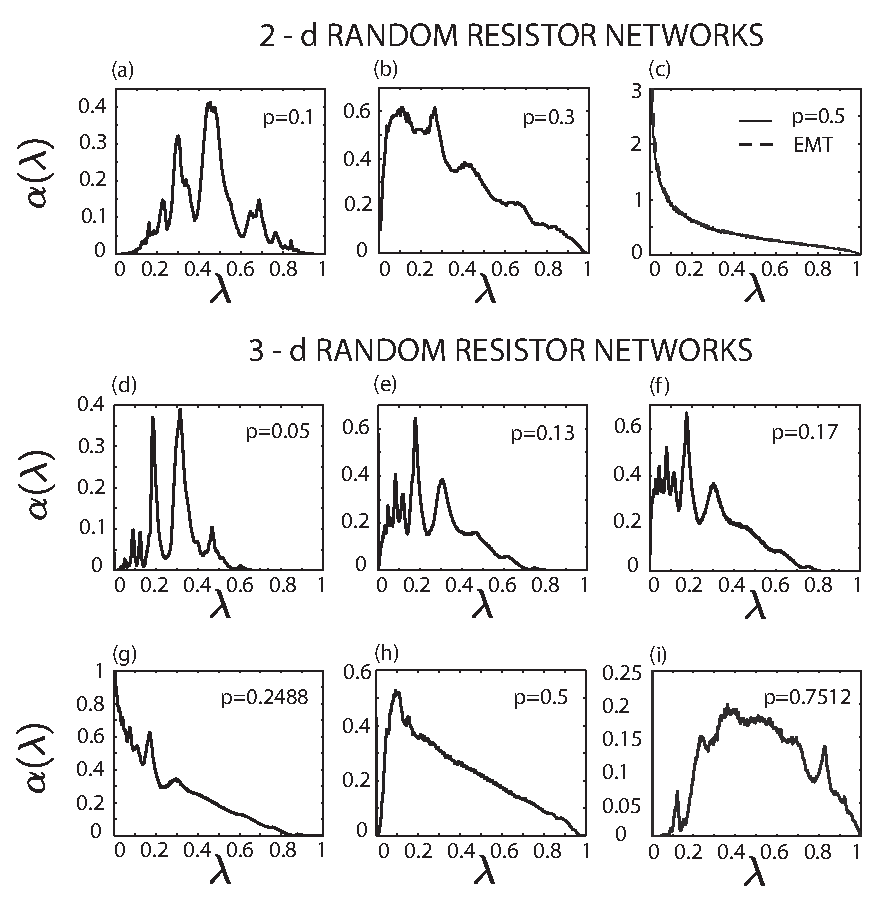
\includegraphics[width=35pc]{2-3-d_Random_Resistor_Networks.eps}%
\caption{\emph{The spectral function for the 2--d and 3--d square random bond
    networks.} As the volume fraction $p$ of defect bonds increases,
  from left to right, the width of the gaps in the spectrum near
  $\lambda=0,1$ shrink to 0 with increasing connectedness as the percolation
  thresholds $p_c=0.5$ and $p_c\approx0.2488$ are approached.}%
\end{figure}
%
We now discuss the gaps $\theta_\alpha$ and $\theta_\eta$ (for $p<p_c$), and $\theta_\mu$ and
$\theta_\kappa$ (for $p>p_c$). As the operators $-\Gamma$ and $\Upsilon$ are projectors on
the associated Hilbert spaces $\mathscr{H}_\times$ and $\mathscr{C}_\bullet$,
respectively, the eigenvalues thereof are confined to the set $\{0,1\}$
\cite{Reed-1980}. The associated operators $\mathbf{M}_j$ and $\mathbf{K}_j$,
$j=1,2$ are positive definite compositions of projection operators,
thus the eigenvalues thereof are confined to the set $[0,1]$
\cite{Golden:CMP-467}.

While, in general, the spectra actually extends all the way
to the spectral endpoints $\lambda=0,1$, the part close to $\lambda=0,1$
corresponds to very large, but very rare connected regions of the
defect inclusions (Lifshitz phenomenon), and is
believed to give exponentially small contributions to the effective
complex conductivity (resistivity), and not
affect power law behavior \cite{Golden:PRL-3935}. In
\cite{Bruno:PRSLA-353} O. Bruno has proven the existence of spectral
gaps in matrix/particle systems with polygonal inclusions, and studied
how the gaps vanishes as the inclusions touch (like $p\to p_c$). In
Figure \ref{fig:2D-RBN}, we give a graphical representation of the
spectral measure $\alpha(d\lambda)$ for finite 2--$d$ and 3--$d$ RBNs
\cite{Golden:JoB:337}. This figure shows that, as $p\to p_c^+$, the width
of the gaps in the spectrum near $\lambda=0,1$ vanish. Our simulations also show
that, as $p$ increases beyond $p_c$, the spectrum piles up at the spectral
endpoints $\lambda=0,1$ until $\Sigma_\alpha=\{0,1\}$, when $p=1$. This behavior is
predicted by our result \eqref{eq:Measure_consistency_condition_h} in
section \ref{sec:Measure_Equivalences}, with weights $m(0)=m(p,0)$ and
$w(0)=w(p,0)$. From equation \eqref{eq:Cond-Insul_Crit_Beh_pc} we see
that the onset of the critical transition (the increase of these
weights from zero) occurs \emph{precisely} at the percolation
threshold $p=p_c$, causing delta function components of the measures
$\mu(d\lambda)$ and $\alpha(d\lambda)$ to be present at $\lambda=0,1$ for all $p>p_c$.  

We now provide a proof, for large but finite lattice systems, of the
existence of spectral gaps in these measures which collapse as $p$
tends towards $p_c$. For lattice systems with a finite number $n$ of
lattice sites, the differential equations in
\eqref{eq:Maxwells_Equations_E} become difference equations
(Kirchoff's laws) \cite{Golden:JMP-5627}. Consequently, the operators
$\mathbf{M}_j$ and $\mathbf{K}_j$, $j=1,2$ are given by $N\times N$
matrices, say \cite{Golden:JoB:337,Golden:JMP-5627}. We focus on 
$\mathbf{M}_2=\chi_2(-\Gamma)\chi_2$, as our results extend to the other operators
by symmetry. In this lattice setting, $-\Gamma$ is a real symmetric projection
matrix and can therefore be diagonalized:
$-\Gamma=\mathbf{Q}\mathbf{D}\mathbf{Q}^T$, where 
$\mathbf{D}$ is a diagonal matrix of zeros and ones and $\mathbf{Q}$
is a real orthogonal matrix.
%$\mathbf{Q}\mathbf{Q}^T=\mathbf{Q}^T\mathbf{Q}=\mathbf{I}_N$, and
%$\mathbf{I}_N$ is the $N\times N$ identity matrix.
More specifically,   
%
\begin{align}
  -\Gamma=\left[
  \begin{matrix}
   \line(1,0){10}\;\vec{q}_1\; \line(1,0){10}\\
   \vdots\\
   \line(1,0){10}\;\vec{q}_N\; \line(1,0){10}     
  \end{matrix}
  \right]
  \left[
  \begin{matrix}
  \mathbf{I}_L & \mathbf{0}\\
  \mathbf{0} & \mathbf{0}
  \end{matrix}
  \right]
  \left[
  \begin{matrix}
   \line(1,0){10}\;\vec{q}_1\; \line(1,0){10}\\
   \vdots\\
   \line(1,0){10}\;\vec{q}_N\; \line(1,0){10}   
  \end{matrix}
  \right]^T
  =
  \left[
  \begin{matrix}
   (\vec{q}_1\cdot\vec{q}_1)_L&(\vec{q}_1\cdot\vec{q}_2)_L&\cdots&(\vec{q}_1\cdot\vec{q}_N)_L\\
   %(\vec{q}_2\cdot\vec{q}_1)_L&(\vec{q}_2\cdot\vec{q}_2)_L&(\vec{q}_2\cdot\vec{q}_3)_L&\cdots\\
   \vdots & \vdots & \ddots  & \vdots\\
   (\vec{q}_N\cdot\vec{q}_1)_L&(\vec{q}_N\cdot\vec{q}_2)_L&\cdots&(\vec{q}_N\cdot\vec{q}_N)_L
  \end{matrix}
  \right],
\end{align}
%
where $0<L<N$ when $N\gg1$, $\mathbf{I}_L$ is the $L\times L$ identity matrix,
$\mathbf{0}$ is a matrix of zeros of arbitrary dimension,
$(\vec{q}_i\cdot\vec{q}_j)_L:=\sum_{l=1}^L(\vec{q}_i)_l(\vec{q}_j)_l$, and
$(\vec{q}_i)_l$ is the $l^{\text{th}}$ component of the vector
$\vec{q}_i\in\mathbb{R}^N$. Here, we consider the case where $N\gg1$ so
that $1\ll L<N$.   

The spectral measure $\alpha(d\lambda)$ of the matrix $\mathbf{M}_2$ is given by
a sum of ``Dirac $\delta$ functions,''
%
\begin{align}\label{eq:Spectral_Function}
  \alpha(d\lambda)=
    \left[\sum_{j=1}^N m_j \delta_{\lambda_j}(d\lambda)\right]d\lambda
      :=\alpha(\lambda)d\lambda,
\end{align}
%
where $\delta_{\lambda_j}(d\lambda)$ is the Dirac delta measure centered at $\lambda_j$,
$m_j=\langle\vec{e}_k^{\;T}[\vec{v}_j\vec{v}_j^{\;T}]\,\vec{e}_k\rangle$, 
$\vec{e}_k$ is a $N$--dimensional vector of ones, and $\lambda_j$ and
$\vec{v}_j$ are the eigenvalues and eigenvectors of $\mathbf{M}_2$,
respectively \cite{Golden:JoB:337}. In this matrix case, the associated Stieltjes
transformation of the measure $\alpha(d\lambda)$ \eqref{eq:Herglotz_Funs_sed_LYRB} is
given by the sum $G(t(s))=\sum_{j=1}^nm_j/(1-s-\lambda_j)$, and $\alpha(\lambda)$ in equation
\eqref{eq:Spectral_Function} is called ``\emph{the spectral
  function},'' which is defined only pointwise on the set of
eigenvalues $\{\lambda_j\}$. In Figure \ref{fig:2D-RBN} we give a graphical
representation of the spectral measure for finite 2--$d$ and 3--$d$
RBNs. It displays linearly connected peaks of histograms with bin
sizes on the order of $10^{-2}$. The apparent smoothness of the
spectral function graphs in this figure is due to the large number
($\sim10^6$) of eigenvalues and eigenvectors calculated, and ensemble
averaged. 

In the matrix case, the action of $\chi_2$ is given by that of a square
diagonal matrix of zeros and ones \cite{Golden:JoB:337}. The action
of $\chi_2$ in the matrix $\chi_2(-\Gamma)\chi_2$ introduces a row and column
of zeros in the matrix $-\Gamma$, corresponding to every diagonal entry of
$\chi_2$ with value 0. When there is only one defect inclusion, $p=1/n$,
located at the $j^{\text{th}}$ bond, $\chi_2$ has all zero entries except
at the $j^{\text{th}}$ diagonal:
$\chi_2=\text{diag}(0,\cdots,0,1,0,\cdots,0):=\text{diag}(\vec{\text{v}}_j)$. Therefore, 
the only non-trivial eigenvalue is given by 
$\lambda_0=(\vec{q}_j\cdot\vec{q}_j)_L=\sum_{l=1}^L(\vec{q}_j)_l^2=1-\sum_{l=L+1}^N(\vec{q}_j)_l^2$, 
with eigenvector $\vec{\text{v}}_j$ and weight $m_0=1/n$. This  
implies that there is a gap at $\lambda=0$, $\theta_0:=\sum_{l=1}^L(\vec{q}_j)_l^2>0$,
and a gap at $\lambda=1$, $\theta_1:=\sum_{l=L+1}^N(\vec{q}_j)_l^2>0$. It is clear
that these bounds hold for all $\omega\in\Omega$ such that $p=1/n$ when $L\gg1$. We
have already mentioned that the eigenvalues of $\mathbf{M}_1$ are
restricted to the set $\{0,1\}$ when $p=1$
$(\chi_2\equiv\mathbf{I}_N)$. Therefore, there exists $0<p_0<1$ such that,
for all $p\geq p_0$, there exists a $\omega\in\Omega$ such that $\theta_0(\omega)=0$ and/or
$\theta_1(\omega)=0$. %(\textbf{Is it worth doing the 2x2 case?})

% The eigenvalue problem for the case of two defect inclusions at the
% $i^{th}$ and $j^{th}$ bond is given by that of a $2\times2$ symmetric
% matrix. In this case, the non--trivial part of the matrix $\chi_2(-\Gamma)\chi_2$
% is given by the matrix 
% % 
% \begin{align}
%   \mathbf{M}_0:=
%   \left[
%     \begin{matrix}
%       (\vec{q}_i\cdot\vec{q}_i)_L&(\vec{q}_i\cdot\vec{q}_j)_L\\
%       (\vec{q}_j\cdot\vec{q}_i)_L&(\vec{q}_j\cdot\vec{q}_j)_L
%     \end{matrix}
%   \right].  
% \end{align}
% The eigenvalues are given by 
% %
% \begin{align}
% \lambda_\pm=\frac{\text{Tr}\mathbf{M}_0}{2}
% \left[1\pm\sqrt{1-\frac{4\text{Det}\mathbf{M}_0}{(\text{Tr}\mathbf{M}_0)^2}}
% \right],  
% \end{align}
% %
% where $\text{Tr}\mathbf{M}_0$ is the trace of $\mathbf{M}_0$ and
% $\text{Det}\mathbf{M}_0$ is the determinant of $\mathbf{M}_0$. By the
% symmetry of $\mathbf{M}_0$, we have $\lambda_\pm\in\mathbb{R}$. Therefore
% $\lambda_+\lambda_-=\text{Det}\mathbf{M}_0<(\text{Tr}\mathbf{M}_0/2)^2<1$, as
% $\lambda_++\lambda_-=\text{Tr}\mathbf{M}_0=(\vec{q}_i\cdot\vec{q}_i)_L+(\vec{q}_j\cdot\vec{q}_j)_L
% =2-\sum_{l=L+1}^N[(\vec{q}_i)_l^2+(\vec{q}_j)_l^2]<2$.
%
\subsection{Baker's Critical Theory for Transport in Binary Composite
  Media}\label{sec:Bakers_Critical_Theory}
%
Baker's critical theory characterizes phase transitions of a given system
via the asymptotic behaviors of underlying Stieltjes functions, near a
critical point. This powerful method has been very successful in the
Ising model, precisely characterizing the phase transition
(spontaneous magnetization) \cite{Baker-1990}.
We now show how this method may be adapted to provide a detailed
description of phase transitions in transport, exhibited by binary
composite media.    
%
% \begin{definition}  \label{def:stieltjes}
%   A function $\zeta(\upsilon)$ is said to be a \emph{Stieltjes function} if 
%   %
%   \begin{align} \label{eq:stieltjes}
%     \zeta(\upsilon)=\int_0^\infty\frac{d\xi(\lambda)}{1+\upsilon\lambda}
%     =\sum_{j =0}^\infty(-\upsilon)^j\int_0^\infty \lambda^jd\xi(\lambda)
%     :=\sum_{j =0}^\infty(-\upsilon)^j\xi_j,
%   \end{align}
%   %
%   where $\xi(\lambda)$ is a bounded, non-decreasing function, taking on
%   infinitely many values, and all the moments $\xi_j$ of $\xi$ are
%   finite.  
% \end{definition}
% %
% By hypothesis, for $p<p_c$ the measure $\ph$ is compactly supported,
% hence bounded with bounded moments of all orders. Therefore the
% function $\hat{g}(h):=\hat{g}(p,h)$ is a Stieltjes function for
% $p<p_c$. For all $h\in\mathcal{U}$ the Stieltjes function $\hat{g}(p,h)$
% is analytic and has a convergent series representation
% \eqref{eq:stieltjes} for all $h\in\mathcal{U}$ such that
% $|h|\hat{S}(p)<1$ \cite{Golden:PRL-3935,Golden:CMP-473}. Similarly for
% $p>p_c$, $g(h):=g(p,h)$ is a Stieltjes function and is analytic
% with a convergent series representation \eqref{eq:stieltjes} for all
% $h\in\mathcal{U}$ such that $|h|S(p)<1$.
%
The following theorem
characterizes Stieltjes functions (series of Stieltjes) \cite{Baker-1990}.  
% 
\begin{theorem} \label{thm:stieltjes_Characterization}
   Let $D(i,j)$ denote the following determinant
    \begin{align} \label{eq:Detf} 
     D(i,j) = \left|
                 \begin{matrix}
                   \xi_i&\xi_{i+1}&\cdots&\xi_{i+j}\\ 
                   \vdots&\vdots&\ddots&\vdots\\
                   \xi_{i+j}&\xi_{i+j+1}&\cdots&\xi_{i+2j}                            
                   \end{matrix}
              \right| .
   \end{align}
   %where $D(i,j)=D(j,i)$.
   The $\xi_n$ form a series of Stieltjes if and only if
   $D(i,j) \geq 0$ for all $i,j =0,1,2,\ldots$ 

 \end{theorem} 
%
Baker's inequalities for the sequences $\gamma_n$
\eqref{eq:Crit_Exponents_mh} and $\gh_n$ \eqref{eq:Crit_Exponents_wh}
of transport follow from Theorem
\ref{thm:stieltjes_Characterization}. Indeed, 
for example, $\phi_n\sim(p-p_c)^{-\gamma_n}$ and Theorem
\ref{thm:stieltjes_Characterization} with $\phi_i=\xi_i$, $i=n$, and $j=1$,
imply that, for $|p-p_c|\ll1$,
%
\begin{align} \label{eq:CondBakerIneq_m}
  &(p-p_c)^{-\gamma_n - \gamma_{n+2}}-(p-p_c)^{-2\gamma_{n+1}} \geq  0
  %\notag \\
%  
  \iff (p-p_c)^{-\gamma_n - \gamma_{n+2} + 2\gamma_{n+1} }\geq1
%  \notag \\
%  
  \notag\\&\iff -\gamma_n - \gamma_{n+2} + 2\gamma_{n+1} \leq 0
%  \notag\\
%  
  \iff  \boxed{ \gamma_{n+1}-2\gamma_n+\gamma_{n-1}\geq  0}\,.
\end{align}
% 
The sequence of inequalities \eqref{eq:CondBakerIneq_m} are
\emph{Baker's inequalities} for transport, corresponding to $m(p,h)$,
and they imply that the sequence $\gamma_n$ increases at least linearly
with $n$.  The symmetries in equations \eqref{eq:mh_Stieltjes_rep} and
\eqref{eq:Crit_Exponents_mh}--\eqref{eq:Crit_Exponents_wh} imply that
Baker's inequalities also hold for the sequences $\gamma_n^\prime$, $\gh_n$, and
$\gh_n^\prime$. 
%--------------------------------------------------------------------
\begin{lemma}\label{lem:h_diff_commutation}
   Let $0<h\ll1$ and $|p-p_c|\ll1$. Then the integrals in equation
   \eqref{eq:Integral_rep_g_ghat} have the following asymptotics for $n\geq0$
%  .
\begin{align}\label{eq:Diff_g}
  &\frac{\partial^ng(p,h)}{\partial h^n}\sim\phi_n, \qquad \frac{\partial^n\hat{g}(p,h)}{\partial h^n}\sim\ph_n.
\end{align}
\end{lemma}
%
\noindent \textbf{Proof}:
%
The asymptotic behaviors in equation
\eqref{eq:Diff_g} follow from equations
\eqref{eq:phi_moments}--\eqref{eq:phi_moments_F(s)},
\eqref{eq:phi_hat_moments}, Baker's inequalities
\eqref{eq:CondBakerIneq_m}, and equation \eqref{eq:mh_Stieltjes_rep}
 ($g(p,h)=sF(p,s)$ and $\hat{g}(p,h)=-s\,G(p,t(s))$).
They imply that, for $c_j,b_j\in\mathbb{Z}$,  
%
\begin{align*}%\label{eq:Diff_mh_Fs}
  &\lim_{h\to0}\frac{\partial^ng(p,h)}{\partial h^n}
         =\sum_{j=0}^nc_j\lim_{s\to1}\frac{\partial^jF(p,s)}{\partial s^j}\sim\phi_n\,,
  &&
  \lim_{h\to0}\frac{\partial^n\hat{g}(p,h)}{\partial h^n}
         =\sum_{j=0}^nb_j\lim_{s\to1}\frac{\partial^jG(p,t(s))}{\partial t^j}\sim\ph_n\, \ \Box.      
\end{align*}
%-----------------------------------------------------------------------

The key results of this section are the two--parameter scaling
relations between the critical exponents in the conductor/insulator
system, defined in equations \eqref{eq:Crit_Exponents_mh},
and that of the conductor/superconductor system,
defined in equations \eqref{eq:Crit_Exponents_wh}.
By equation \eqref{eq:m_w_relation} we know that $m(p,h)$ and $w(p,z(h))$
are related, therefore the Stieltjes functions $g(p,h)$ and
$\hat{g}(p,h)$ are related. Moreover by equation
\eqref{eq:BM_measure_relationship}, we know that the measures $\mu$ and
$\alpha$ are related, therefore the measures $\phi$ and $\ph$ are related. We
therefore anticipate that these two sets of critical exponents
% defined in equations \eqref{eq:Crit_Exponents_mh} and  
% \eqref{eq:Crit_Exponents_wh}
are also related. This is indeed the case, and the resultant
relationship between the critical exponents $t$ and $s$ is in
agreement with the seminal paper by A. L. Efros and B. I. Shklovskii
\cite{Efros:PSSB-303}. These results are summarized in Theorem
\ref{thm:Crit_Theory_m_w} below. 
%
% The key results of this section are the two--parameter scaling
% relations between the critical exponents defined in equations
% \eqref{eq:Crit_Exponents_mh}--\eqref{eq:Crit_Exponents_wh}. These
% results are summarized in Theorem \ref{thm:Crit_Theory_m_w} below.
%
%
\begin{theorem} \label{thm:Crit_Theory_m_w}
  Let $t$, $t_r$, $t_i$, $\delta$, $\delta_r$, $\delta_i$, $\gamma$, $\gamma_n$, $\Delta$, $\gamma_n^\prime$,
  and $\Delta^\prime$ be   defined as in equations \eqref{eq:Crit_Exponents_mh},
  and $s$, $s_r$, $s_i$, $\dha$, $\dha_r$, $\dha_i$, $\gh^\prime$, $\gh_n^\prime$,
  $\Dh^\prime$, $\gh_n$, and $\Dh$ be defined as in equations
  \eqref{eq:Crit_Exponents_wh}. Then the following scaling relations
  hold:
%  
  \begin{align*}   
   &\mathbf{1)} \ \gamma_1=\gamma, \ \gamma_1^\prime=\gamma^\prime, \ \gh_1=\gh, \text{ and } \ \gh_1^\prime=\gh^\prime. \qquad
     \mathbf{2)} \ \gamma_0^\prime=0, \ \gamma_0<0, \ \gamma_n^\prime>0 \text{ and } \gamma_n>, \ n\geq1.\\
   &\mathbf{3)} \ \gh_n^\prime>0 \text{ for } n\geq0. \qquad
   \mathbf{4)} \ \gamma=\gh_0 \text{ and } \Delta=\Dh. \qquad
   \mathbf{5)} \ \gamma^\prime=\gh_0^\prime \text{ and } \Delta^\prime=\Dh^\prime. \\
   &\mathbf{6)} \ \gamma_n=\gamma+\Delta(n-1) \text{ for } n\geq1. \qquad
   \mathbf{7)} \ \gh_n^\prime=\gh_0^\prime+\Dh^\prime n=\gh^\prime+\Dh^\prime(n-1) \text{ for } n\geq0. \\
   &\mathbf{8)} \ t=\Delta-\gamma. \qquad 
   \mathbf{9)} \ s=\gh_0^\prime=\gh^\prime-\Dh^\prime. \qquad
   \mathbf{10)} \ \delta=\frac{\Delta}{\Delta-\gamma}\,. \qquad
   \mathbf{11)} \ \dha\;^\prime=\frac{\Dh^\prime}{\gh_0^\prime}=\frac{\Dh^\prime}{\gh^\prime-\Dh^\prime}\,. \\
   &\mathbf{12)} \ t_r=t_i=t. \qquad
   \mathbf{13)} \ s_r=s_i=s. \qquad
   \mathbf{14)}  \ \delta_r=\delta_i=\delta\,. \qquad
   \mathbf{15)} \ \dha_r=\dha_i=\dha. \\
   &\mathbf{16)} \text{ If } \Delta=\Delta^\prime \ \text{ and } \ \gamma=\gamma^\prime, \ \text{
     then } \ t+s=\Delta \ \text{ and } \ 1/\delta+1/\dha\,^\prime=1.
  \end{align*}
%  
\end{theorem}
%

Theorem \ref{thm:Crit_Theory_m_w} will be proven via a sequence of
lemmas as we collect some important properties of $m(p,h)$, $g(p,h)$,
$w(p,z(h))$, and $\hat{g}(p,h)$, and how they are related.
%----------------------------------------------------------------
\begin{lemma}\label{lem:nonzero_gamma1_etc}
  $\gamma_1=\gamma$, $\gamma_1^\prime=\gamma^\prime$, $\gh_1=\gh$, and $\gh_1^\prime=\gh^\prime$
\end{lemma}
%
\noindent \textbf{Proof}:
%
Set $0<p-p_c\ll1$. By equations \eqref{eq:mh_Stieltjes_rep}
$(g(p,h)=sF(p,s))$, \eqref{eq:phi_moments_F(s)},
\eqref{eq:Crit_Exponents_mh}, and \eqref{eq:CondBakerIneq_m} 
%
\begin{align}\label{eq:gamma1_gamma}
  (p-p_c)^{-\gamma}\sim\chi(p,0)
          :=\frac{\partial m(p,0)}{\partial h}
          =\lim_{s\to1}\left[-\frac{\partial F(p,s)}{\partial s}\right]
          =\phi_0+\phi_1
          \sim\phi_1\sim(p-p_c)^{-\gamma_1},
\end{align}
%
hence $\gamma_1=\gamma$. Similarly for $0<p_c-p\ll1$, we have $\gamma_1^\prime=\gamma^\prime$. By
equation \eqref{eq:gamma1_gamma}, the symmetries between $m$ and
$w$ \eqref{eq:mh_Stieltjes_rep} and the critical exponent definitions 
\eqref{eq:Crit_Exponents_mh}--\eqref{eq:Crit_Exponents_wh}, we also
have $\gh_1=\gh$ and $\gh_1^\prime=\gh^\prime$ $\Box$.   
%----------------------------------------------------------------

Equation \eqref{eq:m_w_relation} is consistent with, and provides a
link between equations \eqref{eq:Cond-Insul_Crit_Beh_pc} and
\eqref{eq:Cond-SuperCond_Crit_Beh_pc}. We will see that the
fundamental asymmetry  between $m(p,h)$ and $w(p,z(h))$ ($\gamma_0^\prime=0$ and
$\gh_0^\prime>0$), given in Theorem \ref{thm:Crit_Theory_m_w}.2-3, is a
direct and essential consequence of equation \eqref{eq:m_w_relation},
and has deep and far reaching implications.      
%
%----------------------------------------------------------------
\begin{lemma}\label{lem:zero_gamma0}
  %
  Let the sequences $\gamma_n$ and $\gamma_n^\prime$, $n\geq0$, be defined as in
  equation \eqref{eq:Crit_Exponents_mh}. Then
  %
  \begin{align*}
    &\mathbf{1)} \quad \gamma_0^\prime=0, \ \gamma_0<0, \ \gamma_n^\prime>0,   \text{ and } \ \gamma_n>0, \
        \text{ for } \ n\geq1. \\
    &\mathbf{2)} \quad 0<\lim_{h\to0}\langle\chi_1\vec{E}\cdot\vec{E}_0\rangle/E_0^2<1 \
         \text{ for all } \ p\in[0,1], \ h\in\mathcal{U}.
  \end{align*}
  %
\end{lemma}
%
\noindent \textbf{Proof}:
%
By equation \eqref{eq:Cond-SuperCond_Crit_Beh_pc} $|w(p,z(0))|$ is  
bounded for all $p<p_c$. Thus for all $p<p_c$, equations
\eqref{eq:phi_moments_F(s)}, \eqref{eq:m_w_relation},
and \eqref{eq:Crit_Exponents_mh} imply that
%
\begin{align*}
  0=\lim_{h\to0}hw(p,z(h))=\lim_{h\to0}m(p,h)=\lim_{s\to1}(1-F(p,s))=1-\phi_0(p)\sim1-(p_c-p)^{-\gamma_0^\prime},
\end{align*}
%
where the rightmost relation holds for $0<p_c-p\ll1$ and the leftmost
relation is consistent with equation
\eqref{eq:Cond-Insul_Crit_Beh_pc}. Therefore, $\gamma_0^\prime=0$ and $\phi$ is a
probability measure for all $p<p_c$. The strict positivity of the
$\gamma_n^\prime$, for $n\geq1$, follows from Baker's inequalities
\eqref{eq:CondBakerIneq_m}. Thus, from equation
\eqref{eq:gamma1_gamma} we have 
%
\begin{align}\label{eq:div_phi1}
  \infty=\lim_{p\to p_c^-}\phi_1(p)=-\lim_{p\to p_c^-}\frac{\partial m(p,0)}{\partial h}\,.
\end{align}
%

For $p>p_c$, equations \eqref{eq:phi_moments_F(s)} and
\eqref{eq:Cond-Insul_Crit_Beh_pc} imply that
$0<\lim_{h\to0}|m(p,h)|=1-\phi_0<1$. Therefore, $(p-p_c)^{-\gamma_0}\sim\phi_0<1$ for
all $0<p-p_c\ll1$, hence $\gamma_0<0$. The strict positivity of $\gamma_1$ follows
from equation \eqref{eq:div_phi1}, and the strict positivity of the
$\gamma_n$ for $n\geq2$ follows from Baker's inequalities
\eqref{eq:CondBakerIneq_m}. Equation \eqref{eq:phi_energy_relations}
and the inequality $0<\lim_{h\to0}|m(p,h)|=1-\phi_0<1$ imply that
$0<\lim_{h\to0}\langle\chi_1\vec{E}\cdot\vec{E}_0\rangle/E_0^2<1$ for all $p\in[0,1]$ $\Box$.    
%    
%------------------------------------------------------
%
%-------------------------------------------------------
\begin{lemma}\label{lem:nonzero_gh_n}
  %
  Let the sequence $\gh_n^\prime$, $n\geq0$, be defined as in equation
  \eqref{eq:Crit_Exponents_wh}. Then
  %
  \begin{align*}
  &\mathbf{1)} \quad \gh_n^\prime>0 \ \text{ for all } \ n\geq0.
  \\%\qquad
  &\mathbf{2)} \quad \lim_{h\to0}\langle E_f^2\rangle=\infty \ \text{ for all } \ p>p_c\,.
  \end{align*}
  %
\end{lemma}
%
\noindent \textbf{Proof}:
%
By equation \eqref{eq:Cond-Insul_Crit_Beh_pc} we have
$0<\lim_{h\to0}|m(p,h)|<1$, for all $p>p_c$. Therefore equation
\eqref{eq:m_w_relation} implies that
$\lim_{h\to0}w(p,z(h))=\lim_{h\to0}m(p,h)/h=\infty$, for all $p>p_c$, which is
consistent with equation
\eqref{eq:Cond-SuperCond_Crit_Beh_pc}. More specifically, for all
$p>p_c$, equations \eqref{eq:m_w_relation} and
\eqref{eq:Cond-Insul_Crit_Beh_pc} imply that
$0\leq\lim_{h\to0}|m(p,h)|=\lim_{h\to0}|hw(p,z(h))|:=L(p)<1$, where
$L(p)=0$ for all $p<p_c$. Therefore, by equation
\eqref{eq:mh_Stieltjes_rep}, we have
%$\lim_{h\to0}|hw(p,z(h))|=\lim_{h\to0}|h\hat{g}(p,h)|=0$ and
%
\begin{align}\label{eq:Divergence_Rate_w(p,z(h))}
  &\lim_{h\to0}|h\,w(p,z(h))|=\lim_{h\to0}|h\,\hat{g}(p,h)|\in(0,1), 
                        \text{ for all } p>p_c, 
 \\
  &\lim_{h\to0}|h\,w(p,z(h))|=\lim_{h\to0}|h\,\hat{g}(p,h)|=0,
         \text{ for all } p< p_c \,. \notag                                       
\end{align}
%
%As will be shown below, equation \eqref{eq:Divergence_Rate_w(p,z(h))} has
%very important consequences.
By equations \eqref{eq:phi_hat_moments},
\eqref{eq:Cond-SuperCond_Crit_Beh_pc}, and
\eqref{eq:Crit_Exponents_wh} we have, for all $p>p_c$,
%
\begin{align*}
  \infty=\lim_{p\to p_c^-}\lim_{h\to0}w(p,z(h))
   =\lim_{p\to p_c^-}\lim_{s\to1}(1-G(p,t(s)))
   =1+\lim_{p\to p_c^-}\ph_0(p)
   \sim1+\lim_{p\to p_c^-}(p_c-p)^{-\gh_0^\prime},
\end{align*}
%
hence $\gh_0^\prime>0$. Baker's inequalities \eqref{eq:CondBakerIneq_m}
then imply that $\gh_n^\prime>0$ for all $n\geq0$. Equations
\eqref{eq:phi_energy_relations} and
\eqref{eq:Divergence_Rate_w(p,z(h))}, and $\gh_0^\prime>0$ imply that
$\lim_{h\to0}\langle E_f^2\rangle=\infty$ for all $p>p_c$ $\Box$.
%   
%----------------------------------------------------------------------

The asymptotic behavior of $\hat{g}(p,h)$ in equation
\eqref{eq:Diff_g}, and Lemma \ref{lem:nonzero_gh_n} motivates 
the following fundamental homogenization assumption of this section
\cite{Baker-1990}:   
%
\begin{remark}\label{rem:homogenization_w}
Near the critical point $(p,h)=(p_c,0)$, the asymptotic behavior of
the Stieltjes function $\hat{g}(p,h)$ is determined primarily by the
mass $\ph_0(p)$ of the measure $\ph$ and the rate of collapse of the
spectral gap $\theta_\alpha$.  
\end{remark}
%
\noindent By remark \ref{rem:homogenization_w}, and in light of Lemmas
\ref{lem:nonzero_gamma1_etc}--\ref{lem:nonzero_gh_n}, we make the
following variable changes:
%
\begin{align}\label{eq:variable_change_w}
  &\qh:=y(p_c-p)^{\Dh^\prime}, && \hat{Q}(p):=\hat{S}(p)(p_c-p)^{\Dh^\prime},
      %\quad x:=h(p-p_c)^{\Dh^\prime},\\
      && d\hat{\pi}(\qh):=(p_c-p)^{\gh_0^\prime} \;d\ph(y),
  \\
  %\label{eq:variable_change_m}
   &q:=y(p-p_c)^\Delta, && Q(p):=S(p)(p-p_c)^\Delta,
      %\quad x:=h(p-p_c)^{\Dh},\\
      && d\pi(q):=(p-p_c)^\gamma \;y\,d\ph(y), \notag
\end{align}
%
so that, by equations
\eqref{eq:Crit_Exponents_mh}--\eqref{eq:Crit_Exponents_wh},
$\hat{Q}(p),Q(p)\sim1$ and the masses $\hat{\pi}_0$ and $\pi_0$ of the
measures $\hat{\pi}$ and $\pi$, respectively, satisfy $\hat{\pi}_0,\pi_0\sim1$ as
$p\to p_c$. 

Equation \eqref{eq:variable_change_w}
defines the following scaling functions $G_{n-1}(x)$, $\hat{G}_n(\xh)$,
$\mathcal{G}_{n-1,j}(x)$, and $\hat{\mathcal{G}}_{n,j}(\xh)$ as follows.
For $h\in\mathcal{U}\cap\mathbb{R}$, equations \eqref{eq:Integral_rep_g_ghat} and 
\eqref{eq:variable_change_w} imply, for 
$n\geq0$, that       
%
\begin{align}\label{eq:Scaling_fun_Def}
  &\frac{\partial^ng}{\partial h^n}\propto(p-p_c)^{-(\gamma+\Delta(n-1))} G_{n-1}(x),
      %&=\int_0^{S(p)}\frac{y^n d\phi(y)}{(1+hy)^{n+1}}
      %=(p_c-p)^{-(\gamma+\Delta n)}\int_0^{Q(p)}
      %   \frac{q^n d\pi(q)}{(1+xq)^{(n+1)}}\\
%     
&&
  \frac{\partial^n\hat{g}}{\partial h^n}\propto(p_c-p)^{-(\gh_0^\prime+\Dh^\prime n)} \hat{G}_n(\xh), 
      %&=\int_0^{\hat{S}(p)}\frac{y^nd\ph(y)}{(1+hy)^{n+1}}
      %=(p_c-p)^{-(\gh_0^\prime+\Dh^\prime n)}\int_0^{\hat{Q}(p)}
      %   \frac{\qh^nd\hat{\pi}(\qh)}{(1+xq)^{(n+1)}}\\
\\ 
  &G_{n-1}(x):=\int_0^{Q(p)}\frac{q^{n-1}d\pi(q)}{(1+xq)^{n+1}},
&&
  \hat{G}_n(\xh):=\int_0^{\hat{Q}(p)}\frac{\qh^{\,n}d\hat{\pi}(\qh)}{(1+\xh \qh)^{n+1}},
\notag\\  
  &x:=h(p-p_c)^{-\Delta}, \quad 0<p-p_c\ll1,
  &&
  \xh:=h(p_c-p)^{-\Dh^\prime}, \quad 0<p_c-p\ll1. \notag
\end{align}
%
Analogous formulas are defined for the opposite limits involving
$\Dh$, $\gh_0$, $\Delta^\prime$, and $\gamma^\prime$. 

For $h\in\mathcal{U}$ such that $h_i\neq0$, we define the scaling
functions $\mathcal{R}_{n-1}(x)$, $\mathcal{I}_{n-1}(x)$,
$\hat{\mathcal{R}}_{n}(\xh)$, and $\hat{\mathcal{I}}_{n}(\xh)$ as
follows. Using equations \eqref{eq:Complex_Diff_g} and
\eqref{eq:variable_change_w} we have,
for $0<p-p_c\ll1$,  
%
\begin{align}\label{eq:Complex_Scaling_fun_Def}
\frac{\partial^ng}{\partial h^n}   
   &=(-1)^nn!\sum_{j=0}^{n+1}{n+1 \choose j}\bar{h}^j
                 \int_0^{S(p)}\frac{y^{n+j}d\phi(y)}{|1+hy|^{2(n+1)}}\\
   &:=(-1)^nn!\sum_{j=0}^{n+1}{n+1 \choose j}[\bar{x}(p-p_c)^\Delta]^j
                 (p-p_c)^{-(\gamma+\Delta(n-1+j))}\mathcal{G}_{n-1,j}(x)\notag\\
   &:=(-1)^nn!(p-p_c)^{-(\gamma+\Delta(n-1))}\mathcal{K}_{n-1}(x), \quad
   \mathcal{K}_{n-1}(x):=\mathcal{R}_{n-1}(x)+\I\,\mathcal{I}_{n-1}(x),
   \notag\\
   %&:=(-1)^nn!(p-p_c)^{-(\gamma+\Delta(n-1))}
   %   \left[\mathcal{R}_{n-1}(x)+\I\,\mathcal{I}_{n-1}(x)\right],
   %\text{ and similarly}, \notag\\
\frac{\partial^n\hat{g}}{\partial h^n}
     &:=(-1)^nn!(p-p_c)^{-(\gh_0+\Dh n)}\hat{\mathcal{K}}_n(\xh), \quad
       \hat{\mathcal{K}}_n(\xh):=\hat{\mathcal{R}}_{n}(\xh)+\I\,\hat{\mathcal{I}}_{n}(\xh).
       \notag
\end{align}
%
Here, $x$ and $\xh$ are defined in equation \eqref{eq:Scaling_fun_Def}
and  
%
\begin{align}\label{eq:Complex_Scaling_fun_Def_Integrals}
 &\mathcal{G}_{n-1,j}(x):=\int_0^{Q(p)}\frac{q^{n-1+j}d\pi(q)}{|1+xq|^{2(n+1)}}\,,
 &&
 \hat{\mathcal{G}}_{n,j}(\xh):=\int_0^{\hat{Q}(p)}\frac{\qh^{\,n+j}d\hat{\pi}(\qh)}{|1+\xh\qh|^{2(n+1)}}\,,
 \\
 &\mathcal{K}_{n-1}(x):=\sum_{j=0}^{n+1}{n+1 \choose j}\bar{x}^{\,j}
                       \mathcal{G}_{n-1,j}(x),
 &&
 \hat{\mathcal{K}}_n(\xh):=\sum_{j=0}^{n+1}{n+1 \choose j}\bar{\xh}^j
                       \hat{\mathcal{G}}_{n,j}(\xh),
 \notag
% \\
% &\mathcal{R}_{n-1}(x):=\text{Re}(\mathcal{K}_{n-1}(x)),
% &&
% \hat{\mathcal{R}}_n(\xh):=\text{Re}(\hat{\mathcal{K}}_n(\xh)),
%   \notag\\   
% &\mathcal{I}_{n-1}(\xh):=\text{Im}(\mathcal{K}_{n-1}(x)),
% &&
% \hat{\mathcal{I}}_n(\xh):=\text{Im}(\hat{\mathcal{K}}_n(\xh)),
% \notag
\end{align}
%
where we have made the definitions
$\mathcal{R}_{n-1}(x):=\text{Re}(\mathcal{K}_{n-1}(x))$,
$\mathcal{I}_{n-1}(\xh):=\text{Im}(\mathcal{K}_{n-1}(x))$,
$\hat{\mathcal{R}}_n(\xh):=\text{Re}(\hat{\mathcal{K}}_n(\xh))$, and
$\hat{\mathcal{I}}_n(\xh):=\text{Im}(\hat{\mathcal{K}}_n(\xh))$. Analogous
formulas are defined for the opposite limit, $0<p_c-p\ll1$, involving
$\Dh^\prime$, $\gh^\prime_0$, $\Delta^\prime$, and $\gamma^\prime$.  

From equation \eqref{eq:Herglotz_Inneq} we have, for $h\in\mathcal{U}$,
$p\in[0,1]$, and $n\geq0$, 
%
\begin{align}\label{eq:Non-negative_Gn_Ghn}
   G_{n-1}(x)>0, \quad \mathcal{G}_{n-1,j}(x)>0,\qquad
%
  \hat{G}_n(\xh)>0, \quad  \hat{\mathcal{G}}_{n,j}(\xh)>0. 
\end{align}
%
By our gap hypothesis, the $h$ derivatives of $g(p,h)$ and
$\hat{g}(p,h)$, of all orders, are bounded at $h=0$ for $p>p_c$ and
$p<p_c$\,, respectively.
%(\cite{Golden:CMP-473,Golden:CMP-467,Golden:SIAM89} and references
%therein)).
Therefore, 
% 
\begin{align}\label{eq:Bounded_Gn_h}
  &\lim_{h\to0}G_{n-1}(x)<\infty, &&
  \lim_{h\to0}\mathcal{G}_{n-1,j}(x)<\infty,  &&
  \text{ for all } \ p>p_c, \ \ n\geq0\\
%
  &\lim_{h\to0}\hat{G}_n(\xh)<\infty, &&
  \lim_{h\to0}\hat{\mathcal{G}}_{n,j}(\xh)<\infty,  &&
  \text{ for all } \ p<p_c,\ \ n\geq0. \notag
\end{align}
%
%-----------------------------------------------------------------------------------
 \begin{lemma}\label{lem:asymp_Scaling_funs_x_to_0_p>pc}
   Let $\hat{G}_n(\xh)$, $G_{n-1}(x)$, and the associated critical
   exponents be defined as in equation \eqref{eq:Scaling_fun_Def}, for
   $p>p_c$. Then  
   %
   \begin{align*}
    &\mathbf{1)} \quad G_{n-1}(x)\sim1 \ \text{ as } \ x\to0 \ (h\to0 \
    \text{ and } \ 0<p-p_c\ll1) \ \text{ for all } \ n\geq1. \\
    &\mathbf{2)} \quad [\hat{G}_{n-1}(\xh)-\xh\hat{G}_n(\xh)]\sim1
      %\iff \xh^n\hat{G}_n(\xh)\sim\hat{G}_0(\xh)
       \ \text{ as } \ \xh\to0 \ (h\to0 \text{ and } 0<p-p_c\ll1) \ \text{ for all
         } \ n\geq1.  \\
    &\mathbf{3)} \quad \gamma=\gh_0\,. \\%\qquad
    &\mathbf{4)} \quad \Delta=\Dh\,.    
   \end{align*}
   %
 \end{lemma}
%
\noindent \textbf{Proof}:
%
Let $h\in\mathcal{U}\cap\mathbb{R}$ and $p>p_c.$
%, so that $g(p,h)$ and $\hat{g}(p,h)$ are real analytic
%\cite{Golden:CMP-473}, and $p>p_c$. so that, by equation
%\eqref{eq:Bounded_Gn_h}, all $h$ derivatives of $g(p,h)$ are bounded
%for $h=0$. Therefore,
Equations \eqref{eq:Diff_g_ghat_relation_Integral},
\eqref{eq:Scaling_fun_Def}, and
\eqref{eq:Non-negative_Gn_Ghn}--\eqref{eq:Bounded_Gn_h} imply that we
have, for all $n\geq1$, $0<p-p_c\ll1$, and $0<h\ll1$,    
%
\begin{align}\label{eq:Matching_Condition_Gn_Gnhat_p>pc}
  (0,\infty)\ni(p-p_c)^{-(\gamma+\Delta(n-1))}G_{n-1}(x)
       =(p-p_c)^{-(\gh_0+\Dh(n-1))}[\hat{G}_{n-1}(\xh)-\xh\hat{G}_n(\xh)].
\end{align}
%
Equations \eqref{eq:Non-negative_Gn_Ghn}--\eqref{eq:Bounded_Gn_h}
imply that $G_{n-1}(x)\sim1$ as $x\to0$, for all $n\geq1$. Equation
\eqref{eq:Matching_Condition_Gn_Gnhat_p>pc} then implies that 
$[\hat{G}_{n-1}(\xh)-\xh\hat{G}_n(\xh)]\sim1$ as $\xh\to0$,
for all $n\geq1$ (a competition in sign between two diverging
terms). Or equivalently, generalizing
\eqref{eq:Divergence_Rate_w(p,z(h))},
$\hat{G}_0(\xh)-\xh^n\hat{G}_n(\xh)\sim1$. Therefore,   
%
\begin{align}
  \gamma+\Delta(n-1)=\gh_0+\Dh(n-1), \quad n\geq1.
\end{align}
%
Which in turn, implies that $\gamma=\gh_0$ and $\Delta=\Dh$ $\Box$.
%
%-------------------------------------------------------
%
%-------------------------------------------------------
 \begin{lemma}\label{lem:asymp_Scaling_funs_x_to_0_p<pc}
   Let $\hat{G}_n(\xh)$, $G_{n-1}(x)$, and the associated critical
   exponents be defined as in equation \eqref{eq:Scaling_fun_Def}, for
   $p<p_c$. Then
   %
     \begin{align*}
    &\mathbf{1)}\quad \hat{G}_{n-1}(\xh)\sim1 \ \text{ as } \ \xh\to0 \ (h\to0
    \ \text{ and } \ 0<p_c-p\ll1), \ \text{ for all } \ n\geq1. \\
    &\mathbf{2)}\quad G_{n-1}(x)\sim1 \ \text{ as } \ x\to0 \ (h\to0 \ \text{
      and } \ 0<p_c-p\ll1, \ \text{ for all } \ n\geq1.\\
    &\mathbf{3)}\quad \gamma^\prime=\gh_0^\prime.  \\%\qquad
    &\mathbf{4)}\quad \Delta^\prime=\Dh^\prime.   
     \end{align*}
   %
 \end{lemma}
%
\noindent \textbf{Proof}:
%
Let $h\in\mathcal{U}\cap\mathbb{R}$ and $p<p_c$.
%, so that $g(p,h)$ and $\hat{g}(p,h)$ are
%real analytic \cite{Golden:CMP-473}. Moreover let $p<p_c$ so that, by
%equation \eqref{eq:Bounded_Gn_h}, all $h$ derivatives of
%$\hat{g}(p,h)$ are bounded for $h=0$. Thus
%By equations \eqref{eq:Integral_rep_g_ghat} and \eqref{eq:Bounded_Gn_h} we
%have the following: $\lim_{h\to0}h \int_0^{S(p)}y^nd\ph(y)/(1+hy)^{n+1}=0$. 
Equations \eqref{eq:Diff_g_ghat_relation_Integral}, 
\eqref{eq:Scaling_fun_Def}, and
\eqref{eq:Non-negative_Gn_Ghn}--\eqref{eq:Bounded_Gn_h} imply that,
for all $n\geq1$, $0<p_c-p\ll1$, and $0<h\ll1$,  
% %
% \begin{align}\label{eq:Matching_Condition_Gn_Gnhat_p<pc}
%   (0,\infty)\ni(p_c-p)^{-(\gh^\prime+\Dh^\prime(n-1))}\hat{G}_{n-1}(\xh)
%        \sim(p_c-p)^{-(\gamma^\prime+\Delta^\prime(n-1))}G_{n-1}(x).
% \end{align}
% %
%
\begin{align}\label{eq:x_infty_p<pc}
  (0,\infty)\ni(p_c-p)^{-(\gh_0^\prime+\Dh^\prime(n-1))}[\hat{G}_{n-1}(\xh)-\xh\hat{G}_n(\xh)]
       =(p_c-p)^{-(\gamma^\prime+\Delta^\prime(n-1))}G_{n-1}(x)
\end{align}
%
Equations \eqref{eq:Non-negative_Gn_Ghn}--\eqref{eq:Bounded_Gn_h}
imply that $\hat{G}_{n-1}(\xh)\sim1$ as $\xh\to0$ for all $n\geq1$. Equation 
\eqref{eq:x_infty_p<pc} then implies that
$G_{n-1}(x)\sim1$ as $x\to0$ for all $n\geq1$. Therefore, 
%
\begin{align*}
  \gamma^\prime+\Delta^\prime(n-1)=\gh_0^\prime+\Dh^\prime(n-1), \quad n\geq1.
\end{align*}
%
Which in turn, implies that $\gamma^\prime=\gh_0^\prime$ and $\Delta^\prime=\Dh^\prime$ $\Box$.
%
%-------------------------------------------------------
%
%-------------------------------------------------------
 \begin{lemma}\label{lem:Scaling_rel_t_s_gamman}
   Let $\hat{G}_n(\xh)$, $G_{n-1}(x)$, and the associated critical
   exponents be defined as in equation
   \eqref{eq:Scaling_fun_Def}. Then   
   %
     \begin{align*}
    &\mathbf{1)} \quad \gamma_n= \gamma+\Delta(n-1), \ \text{ for all } \ n\geq1. \\
    &\mathbf{2)} \quad\gh_n^\prime=\gh_0^\prime+\Dh^\prime n=\gh^\prime+\Dh^\prime(n-1), \
    \text{ for all } \ n\geq0. \\
    &\mathbf{3)} \quad t=\Delta-\gamma. \\%\qquad 
    &\mathbf{4)} \quad s=\gh_0^\prime=\gh^\prime-\Dh^\prime.  
     \end{align*}
   %
 \end{lemma}
%
\noindent \textbf{Proof}:
%
Let $0<p-p_c\ll1$. By equations \eqref{eq:Crit_Exponents_mh},
\eqref{eq:Diff_g}, and \eqref{eq:Scaling_fun_Def}, and Lemma  
\ref{lem:asymp_Scaling_funs_x_to_0_p>pc} we have, for all $n\geq1$,
%
\begin{align*}
  (p-p_c)^{-\gamma_n}\sim\phi_n
             \sim\lim_{h\to0}\frac{\partial^ng(p,h)}{\partial h^n}
             \sim(p-p_c)^{-(\gamma+\Delta(n-1))}\lim_{x\to0}G_{n-1}(x)
             \sim(p-p_c)^{-(\gamma+\Delta(n-1))}.\notag 
\end{align*}
%
Therefore $\gamma_n=\gamma+\Delta(n-1)$ for all $n\geq1$, with constant gap
$\gamma_i-\gamma_{i-1}=\Delta$, which is consistent with the absence of multifractal
behavior for the bulk conductivity \cite{Stauffer-92}.

Now let $0<p_c-p\ll1$. By equations \eqref{eq:Crit_Exponents_wh},
\eqref{eq:Diff_g}, and \eqref{eq:Scaling_fun_Def}, and Lemma
\ref{lem:asymp_Scaling_funs_x_to_0_p<pc} we have, for all $n\geq1$, 
%
\begin{align*}
  (p_c-p)^{-\gh_n}\sim\ph_n
             \sim\lim_{h\to0}\frac{\partial^n\hat{g}(p,h)}{\partial h^n}
             \propto(p_c-p)^{-(\gh_0^\prime+\Dh^\prime n)}\lim_{\xh\to0}\hat{G}_n(\xh)
             \sim(p_c-p)^{-(\gh_0^\prime+\Dh^\prime n)}. 
\end{align*}
%
Therefore, by Lemma \ref{lem:nonzero_gamma1_etc}, we have
$\gh_n=\gh_0^\prime+\Dh^\prime n=\gh^\prime+\Dh^\prime(n-1)$ for all $n\geq0$, with constant
gap $\gh^\prime_i-\gh^\prime_{i-1}=\Dh$, which is consistent with the absence of
multifractal behavior for the bulk conductivity \cite{Stauffer-92}.

Again let $0<p-p_c\ll1$. Equations \eqref{eq:mh_Stieltjes_rep},
\eqref{eq:g_ghat_relation}, \eqref{eq:Crit_Exponents_mh}, 
\eqref{eq:Divergence_Rate_w(p,z(h))}, and \eqref{eq:Scaling_fun_Def} yield
%
\begin{align}\label{eq:t_calculation}
  (p-p_c)^t&\sim\lim_{h\to0}m(p,h)
        =1-\lim_{h\to0}g(p,h)
        =\lim_{h\to0}h\hat{g}(p,h)
        =(p-p_c)^{\Dh-\gh_0 }\lim_{\xh\to0}\xh\hat{G}_0(\xh)\notag\\
        &\sim(p-p_c)^{\Dh-\gh_0}.
\end{align}
%
Therefore, by Lemma \ref{lem:asymp_Scaling_funs_x_to_0_p>pc} we have
$t=\Dh-\gh_0=\Delta-\gamma$.

Finally let $0<p_c-p\ll1$. By equations \eqref{eq:mh_Stieltjes_rep}, 
\eqref{eq:Crit_Exponents_wh}, and \eqref{eq:Scaling_fun_Def}, and
Lemmas \ref{lem:nonzero_gh_n} and 
\ref{lem:asymp_Scaling_funs_x_to_0_p<pc}, we have
%
\begin{align*}
  (p_c-p)^{-s}\sim\lim_{h\to0}w(p,z(h))
           \sim\lim_{h\to0}\hat{g}(p,h)
           =(p_c-p)^{-\gh_0^\prime}\lim_{\xh\to0}\hat{G}_0(\xh)
           \sim(p_c-p)^{-\gh_0^\prime}. 
\end{align*}
%
Therefore, by Lemma \ref{lem:Scaling_rel_t_s_gamman}.2, we have
$s=\gh_0^\prime=\gh^\prime-\Dh^\prime$ $\Box$. 
%---------------------------------------------------------------------------
%
%-------------------------------------------------------
 \begin{lemma}\label{lem:G_ghat_asymp_x_to_infty}
   Let $\hat{G}_n(\xh)$, $G_{n-1}(x)$, and the associated critical
   exponents be defined as in equation \eqref{eq:Scaling_fun_Def}, for
   $p>p_c$ and $p<p_c$. Then for all $n\geq1$ 
   %
     \begin{align*}
    &\mathbf{1)} \quad G_{n-1}(x)\sim[\hat{G}_{n-1}(\xh)-\xh\hat{G}_n(\xh)]\sim
      x^{-(\gamma+\Delta(n-1))/\Delta}\,, \text{ as } \xh\to\infty \ (p\to p_c^+  \text{
        and }  0<h\ll1)\,.\\
    &\mathbf{2)} \quad G_{n-1}(x)\sim[\hat{G}_{n-1}(\xh)-\xh\hat{G}_n(\xh)]\sim
      x^{-(\gamma^\prime+\Delta^\prime(n-1))/\Delta^\prime},  \text{ as }  x\to\infty \ (p\to p_c^- 
      \text{ and }  0<h\ll1)\,.\\      
    &\mathbf{3)} \quad \delta=\Delta/(\Delta-\gamma)\,.\\%\qquad
    &\mathbf{4)} \quad \dha\,^\prime=\Dh^\prime/\gh_0^\prime=\Dh^\prime/(\gh^\prime-\Dh^\prime)\,.
     \end{align*}
   %
 \end{lemma}
%
\noindent \textbf{Proof}:
%
Let $0<h\ll1$, so that $g(p,h)$ and $\hat{g}(p,h)$ are analytic for
all $p\in[0,1]$ \cite{Golden:CMP-473}. The analyticity of $g(p,h)$ and
$\hat{g}(p,h)$ implies that all orders of $h$ derivatives of these
functions are bounded as $p\to p_c$, from the left or the
right. Therefore, equation \eqref{eq:Matching_Condition_Gn_Gnhat_p>pc}
holds for $0<p-p_c\ll1$, and equation \eqref{eq:x_infty_p<pc}
holds for $0<p_c-p\ll1$. Moreover, in order to cancel the diverging $p$
dependent 
prefactors in equations \eqref{eq:Matching_Condition_Gn_Gnhat_p>pc}
and \eqref{eq:x_infty_p<pc} we must have, for all $n\geq1$,  
%
\begin{align}\label{eq:Asymp_Gn_Ghn_x_to_infty}
  &G_{n-1}(x)\sim x^{-(\gamma+\Delta(n-1))/\Delta}\,, %\quad
  &&
  [\hat{G}_{n-1}(\xh)-\xh\hat{G}_n(\xh)]\sim\xh^{-(\gh_0+\Dh(n-1))/\Dh}\,, 
      && \text{as } \ p\to p_c^+,
\\
  &G_{n-1}(x)\sim x^{-(\gamma^\prime+\Delta^\prime(n-1))/\Delta^\prime}, %\quad
  &&
  [\hat{G}_{n-1}(\xh)-\xh\hat{G}_n(\xh)]\sim\xh^{-(\gh_0^\prime+\Dh^\prime(n-1))/\Dh^\prime}, 
      && \text{as } \  p\to p_c^-.    \notag
\end{align}
%
Lemma \ref{lem:G_ghat_asymp_x_to_infty}.1-2 follows from equation
\eqref{eq:Asymp_Gn_Ghn_x_to_infty} and Lemmas
\ref{lem:asymp_Scaling_funs_x_to_0_p>pc}--\ref{lem:asymp_Scaling_funs_x_to_0_p<pc}.

Now by equations \eqref{eq:mh_Stieltjes_rep},
\eqref{eq:m_w_relation},
\eqref{eq:Crit_Exponents_mh}, \eqref{eq:Scaling_fun_Def}, and
\eqref{eq:Asymp_Gn_Ghn_x_to_infty} for $n=1$, we have
%
\begin{align}
  h^{1/\delta}&\sim\lim_{p\to p_c^+}m(p,h)
      =\lim_{p\to p_c^+}hw(p,z(h))
      \sim\lim_{p\to p_c^+}h\hat{g}(p,h)
      =h\lim_{p\to p_c^+}(p-p_c)^{-\gh_0 }\hat{G}_0(\xh)\\
      &\sim h(p-p_c)^{-\gh_0 }h^{-\gh_0/\Dh}(p-p_c)^{-\Dh(-\gh_0/\Dh) }
      =h^{(\Dh-\gh_0)/\Dh}. \notag
\end{align}
%
Therefore by Lemma \ref{lem:asymp_Scaling_funs_x_to_0_p<pc}, we have  
$\delta=\Dh/(\Dh-\gh_0)=\Delta/(\Delta-\gamma)$. Similarly by equations
\eqref{eq:mh_Stieltjes_rep}, \eqref{eq:Crit_Exponents_wh},
\eqref{eq:Scaling_fun_Def}, and \eqref{eq:Asymp_Gn_Ghn_x_to_infty}
for $n=1$, and Lemma \ref{lem:nonzero_gh_n}, we have 
%
\begin{align}
   h^{-1/{\dha^\prime}}\sim\lim_{p\to p_c^-}w(p,z(h))
      \sim\lim_{p\to p_c^-}\hat{g}(p,h)
      =\lim_{p\to p_c^-}(p-p_c)^{-\gh_0^\prime}\hat{G}_0(\xh)      
      =h^{-\gh_0^\prime/\Dh\,^\prime}.
\end{align}
%
Therefore, by Lemma \ref{lem:Scaling_rel_t_s_gamman} we have 
$\dha\,^\prime=\Dh^\prime/\gh_0^\prime=\Dh^\prime/(\gh^\prime-\Dh^\prime)$ $\Box$. 
%-------------------------------------------------------
%
%-----------------------------------------------------------------------------------
 \begin{lemma}\label{lem:Complex_s_t}
   Let $h\in\mathcal{U}$ such that $h_i\neq0$, and $\hat{\mathcal{G}}_{n,j}(\xh)$,
   $\hat{\mathcal{R}}_n(\xh)$, $\hat{\mathcal{I}}_n(\xh)$, and the
   associated critical exponents be defined as in equations
   \eqref{eq:Complex_Scaling_fun_Def}--\eqref{eq:Complex_Scaling_fun_Def_Integrals} 
   for $p>p_c$ and $p<p_c$. Furthermore, let $s_r$, $s_i$, $t_r$, and
   $t_i$ be defined as in equations
   \eqref{eq:Crit_Exponents_mh}--\eqref{eq:Crit_Exponents_wh}. Then,       
   %
     \begin{align*}
    &\mathbf{1)} \quad
    [\hat{\mathcal{G}}_{0,0}(\xh)+\xh_r\hat{\mathcal{G}}_{0,1}(\xh)]\sim\xh_i\hat{\mathcal{G}}_{0,1}(\xh)\sim1 
    %\hat{\mathcal{R}}_0(\xh)\sim\hat{\mathcal{I}}_0(\xh)\sim1,
      \ \text{ as }
      \xh\to0 \ (h\to0 \text{ and } \ 0<p_c-p\ll1)\,.\\
    &\mathbf{2)} \quad
      \lim_{\xh\to0}[\xh_r\hat{\mathcal{G}}_{0,0}(\xh)+|\xh|^2\hat{\mathcal{G}}_{0,1}(\xh)]\sim
      \lim_{\xh\to0}[\xh_i\hat{\mathcal{G}}_{0,0}(\xh)]\sim1
      %\lim_{\xh\to0}[\xh_r\hat{\mathcal{R}}_0(\xh)-\xh_i\hat{\mathcal{I}}_0(\xh)]
      %\sim\lim_{\xh\to0}[\xh_r\hat{\mathcal{I}}_0(\xh)+\xh_i\hat{\mathcal{R}}_0(\xh)]\sim1,
      \ \text{ for } \ 0<p-p_c\ll1.  \\
    &\mathbf{3)} \quad s_r=s_i=\gh_0^\prime=s. \\%\qquad
    &\mathbf{4)} \quad t_r=t_i=\Delta-\gamma=t. 
     \end{align*}
   %
 \end{lemma}
%
\noindent \textbf{Proof}:
%
Let $0<p_c-p\ll1$, $h\in\mathcal{U}$ such that $h_i\neq0$, and $0<|h|\ll1$. By
equations
\eqref{eq:Complex_Scaling_fun_Def}--\eqref{eq:Complex_Scaling_fun_Def_Integrals}, 
for $n=0$, we have  
%
\begin{align}
  \hat{g}(p,h)=\int_0^{\hat{S}(p)}\frac{d\ph(y)}{|1+hy|^2}
                +\bar{h}\int_0^{\hat{S}(p)}\frac{y\,d\ph(y)}{|1+hy|^2}
              =(p_c-p)^{-\gh_0^\prime}[\hat{\mathcal{G}}_{0,0}(\xh)
                +\bar{\xh}\hat{\mathcal{G}}_{0,1}(\xh)],
\end{align}
%
so that
%
\begin{align}\label{eq:Complex_ghat}
  \hat{g}_r&=(p_c-p)^{-\gh_0^\prime}\hat{\mathcal{R}}_0(\xh)
          =(p_c-p)^{-\gh_0^\prime}[\hat{\mathcal{G}}_{0,0}(\xh)
                +\xh_r\hat{\mathcal{G}}_{0,1}(\xh)]\\
  \hat{g}_i&=(p_c-p)^{-\gh_0^\prime}\hat{\mathcal{I}}_0(\xh)
          =-(p_c-p)^{-\gh_0^\prime}\xh_i\hat{\mathcal{G}}_{0,1}(\xh).
          \notag
\end{align}
%
Equations \eqref{eq:Divergence_Rate_w(p,z(h))} and \eqref{eq:Non-negative_Gn_Ghn}
imply that $\hat{\mathcal{R}}_0(\xh)\sim\hat{\mathcal{I}}_0(\xh)\sim1$ as
$\xh\to0$ $(h\to0$ and $0<p_c-p\ll1)$. Therefore, equations
\eqref{eq:mh_Stieltjes_rep}, \eqref{eq:Crit_Exponents_wh},
\eqref{eq:Complex_ghat} and Lemma \ref{lem:nonzero_gh_n} imply that 
%
\begin{align}\label{eq:Complex_w_asymp}
  (p_c-p)^{-s_r}&\sim w_r(p,0)
              \sim\hat{g}_r(p,0)
              \sim(p_c-p)^{-\gh_0^\prime}\lim_{\xh\to0}\hat{\mathcal{R}}_0(\xh)
              \sim(p_c-p)^{-\gh_0^\prime},\\
   (p_c-p)^{-s_i}&\sim w_i(p,0)
              \sim\hat{g}_i(p,0)
              \sim(p_c-p)^{-\gh_0^\prime}\lim_{\xh\to0}\hat{\mathcal{I}}_0(\xh)
              \sim(p_c-p)^{-\gh_0^\prime}. \notag            
\end{align}
%
Equation \eqref{eq:Complex_w_asymp} and Lemma
\ref{lem:Scaling_rel_t_s_gamman} imply that $s_r=s_i=\gh_0^\prime=s$. It's
worth noting that these scaling relations are independent of the path
of the limit $h\to0$.  

Now let $0<p-p_c\ll1$ with $h$ as before. In equation
\eqref{eq:t_calculation} we demonstrated
that $m(p,0)=\lim_{h\to0}h\hat{g}(p,h)$. Therefore equation
\eqref{eq:Complex_ghat}, for $p>p_c$, implies that 
%
\begin{align}\label{eq:Complex_ghat_m}
  m_r(p,0)&\sim\lim_{h\to0}[h_r\hat{g}_r(p,h)-h_i\hat{g}_i(p,h)]
         =(p-p_c)^{\Dh-\gh_0}
           %\lim_{\xh\to0}[\xh_r\hat{\mathcal{R}}_0(\xh)-\xh_i\hat{\mathcal{I}}_0(\xh)],
           \lim_{\xh\to0}[\xh_r\hat{\mathcal{G}}_{0,0}(\xh)+|\xh_r|^2\hat{\mathcal{G}}_{0,1}(\xh)]
           \notag\\
  m_i(p,0)&\sim\lim_{h\to0}[h_i\hat{g}_r(p,h)+h_r\hat{g}_i(p,h)]
         =(p-p_c)^{\Dh-\gh_0}
            %\lim_{\xh\to0}[\xh_r\hat{\mathcal{I}}_0(\xh)+\xh_i\hat{\mathcal{R}}_0(\xh)].
            \lim_{\xh\to0}[\xh_i\hat{\mathcal{G}}_{0,0}(\xh)]
\end{align}
%
By equation \eqref{eq:Divergence_Rate_w(p,z(h))} we have
%$\lim_{\xh\to0}[\xh_r\hat{\mathcal{R}}_0(\xh)-\xh_i\hat{\mathcal{I}}_0(\xh)]\sim
%\lim_{\xh\to0}[\xh_r\hat{\mathcal{I}}_0(\xh)-\xh_i\hat{\mathcal{R}}_0(\xh)]\sim1$
$\lim_{\xh\to0}[\xh_r\hat{\mathcal{G}}_{0,0}(\xh)+|\xh|^2\hat{\mathcal{G}}_{0,1}(\xh)]\sim
\lim_{\xh\to0}[\xh_i\hat{\mathcal{G}}_{0,0}(\xh)]\sim1$
for all $0<p-p_c\ll1$. Therefore, equations \eqref{eq:Crit_Exponents_mh} and
\eqref{eq:Complex_ghat_m} imply that
%
\begin{align}\label{eq:Complex_m_asymp}
  &(p-p_c)^{t_r}\sim m_r(p,0)\sim(p-p_c)^{\Dh-\gh_0}, && (p-p_c)^{t_i}\sim m_i(p,0)\sim(p-p_c)^{\Dh-\gh_0}.
\end{align}
%
Equation \eqref{eq:Complex_m_asymp} and Lemmas
\ref{lem:asymp_Scaling_funs_x_to_0_p>pc} and
\ref{lem:Scaling_rel_t_s_gamman} imply that
$t_r=t_i=\Dh-\gh_0=\Delta-\gamma=t$. Again, these scaling relations are
independent of the path of the limit $h\to0$ $\Box$.    
%-----------------------------------------------------------------------------------
%
%-----------------------------------------------------------------------------------
 \begin{lemma} \label{lem:Complex_delta}
   Let $h\in\mathcal{U}$ such that $h_i\neq0$, and $\hat{\mathcal{G}}_{n,j}(\xh)$,
   $\hat{\mathcal{R}}_n(\xh)$, $\hat{\mathcal{I}}_n(\xh)$, and the
   associated critical exponents be defined as in equations
   \eqref{eq:Complex_Scaling_fun_Def}--\eqref{eq:Complex_Scaling_fun_Def_Integrals} 
   for $p>p_c$ and $p<p_c$. Furthermore, let $\dha_r$, $\dha_i$, $\delta_r$, and
   $\delta_i$ be defined as in equations
   \eqref{eq:Crit_Exponents_mh}--\eqref{eq:Crit_Exponents_wh}. Then,       
   %
     \begin{align*}
    &\mathbf{1)} \quad \hat{\mathcal{R}}_0(\xh)\sim\hat{\mathcal{I}}_0(\xh)
                                      \sim|\xh|^{-\gh_0^\prime/\Dh^\prime},
             \text{ as } \xh\to\infty \ (p\to p_c^- \text{ and } 0<|h|\ll1).\\ 
    &\mathbf{2)}\quad
      [\xh_r\hat{\mathcal{R}}_0(\xh)-\xh_i\hat{\mathcal{I}}_0(\xh)]
      \sim[\xh_r\hat{\mathcal{I}}_0(\xh)+\xh_i\hat{\mathcal{R}}_0(\xh)]
      \sim|\xh|^{(\Dh-\gh_0)/\Dh}, \text{ as } \xh\to\infty.    \\
    &\mathbf{3)} \quad \dha_r\,^\prime=\dha_i\,^\prime=\Dh^\prime/\gh_0^\prime=\dha\,.\\%\qquad
    &\mathbf{4)} \quad \delta_r=\delta_i=\Delta/(\Delta-\gamma)=\delta\,. 
     \end{align*}
   %
 \end{lemma}
%
\noindent \textbf{Proof}:
%
Let $h\in\mathcal{U}$ such that $h_i\neq0$ and $0<|h|\ll1$, so that $g(p,h)$
and $\hat{g}(p,h)$ are analytic for all $p\in[0,1]$
\cite{Golden:CMP-473}. Equations \eqref{eq:mh_Stieltjes_rep},
\eqref{eq:Crit_Exponents_wh}, \eqref{eq:Complex_ghat} and Lemma
\ref{lem:nonzero_gh_n} imply that   
%
\begin{align}\label{eq:Complex_w_asymp_infty}
  &|h|^{-1/\dha_r^\prime}\sim w_r(p_c,h)
              \sim\hat{g}_r(p_c,h)
              \sim\lim_{p\to p_c^-}(p_c-p)^{-\gh_0^\prime}\hat{\mathcal{R}}_0(\xh),
              \\
   &|h|^{-1/\dha_i^\prime}\sim w_i(p_c,h)
              \sim\hat{g}_i(p_c,h)
              \sim\lim_{p\to p_c^-}(p_c-p)^{-\gh_0^\prime}\hat{\mathcal{I}}_0(\xh). \notag            
\end{align}
%
The analyticity of $g(p,h)$ and $\hat{g}(p,h)$ implies that they are
bounded for all $p\in[0,1]$. Therefore, in order to cancel the diverging
$p$ dependent prefactors in equations \eqref{eq:Complex_w_asymp_infty}, we
must have
$\hat{\mathcal{R}}_0(\xh)\sim\hat{\mathcal{I}}_0(\xh)\sim|x|^{-\gh_0^\prime/\Dh^\prime}$
as $\xh\to\infty$ $(p\to p_c^-$ and $0<h\ll1)$. Equation
\eqref{eq:Complex_w_asymp_infty} then implies that
%
\begin{align}\label{eq:Complex_}
  &|h|^{-1/\dha_r^\prime}\sim(p_c-p)^{-\gh_0^\prime}|h|^{-\gh_0^\prime/\Dh^\prime}(p_c-p)^{-\Dh^\prime(-\gh_0^\prime/\Dh^\prime)}
               =|h|^{-\gh_0^\prime/\Dh^\prime},&&
   |h|^{-1/\dha_i^\prime}\sim|h|^{-\gh_0^\prime/\Dh^\prime}. %\notag             
\end{align}
%
Therefore, by Lemma \ref{lem:G_ghat_asymp_x_to_infty},
$\dha_r\,^\prime=\dha_i\,^\prime=\Dh^\prime/\gh_0^\prime=\dha\,^\prime$. 

Equations \eqref{eq:mh_Stieltjes_rep} and \eqref{eq:m_w_relation}
imply that $m(p_c,h)\sim\lim_{p\to p_c^+}h\hat{g}(p,h)$, for
$0<|h|\ll1$. Therefore equations \eqref{eq:Crit_Exponents_mh} and
\eqref{eq:Complex_ghat_m} implies that  
%
\begin{align}\label{eq:Complex_ghat_m_infty}
   &|h|^{1/\delta_r}\sim m_r(p_c,h)%&=\lim_{p\to p_c^+}[h_r\hat{g}_r(p,h)-h_i\hat{g}_i(p,h)]\\
         =(p-p_c)^{\Dh-\gh_0}
           \lim_{p\to p_c^+}[\xh_r\hat{\mathcal{G}}_{0,0}(\xh)+|\xh_r|^2\hat{\mathcal{G}}_{0,1}(\xh)],
           \\
  &|h|^{1/\delta_i}\sim m_i(p_c,h)%&=\lim_{p\to p_c^+}[h_r\hat{g}_i(p,h)+h_i\hat{g}_r(p,h)]\notag\\
         =(p-p_c)^{\Dh-\gh_0}
            \lim_{p\to p_c^+}[\xh_i\hat{\mathcal{G}}_{0,0}(\xh)].
            \notag
\end{align}
%
The analyticity of $g(p,h)$ and $\hat{g}(p,h)$ implies that they are
bounded for all $p\in[0,1]$. Therefore, in order to cancel the diverging
$p$ dependent prefactors in equations \eqref{eq:Complex_ghat_m_infty}, we
must have
%$[\xh_r\hat{\mathcal{R}}_0(\xh)-\xh_i\hat{\mathcal{I}}_0(\xh)]
 %\sim[\xh_r\hat{\mathcal{I}}_0(\xh)+\xh_i\hat{\mathcal{R}}_0(\xh)]
$[\xh_r\hat{\mathcal{G}}_{0,0}(\xh)+|\xh_r|^2\hat{\mathcal{G}}_{0,1}(\xh)]\sim
\xh_i\hat{\mathcal{G}}_{0,0}(\xh)\sim|x|^{(\Dh-\gh_0)/\Dh}$
as $\xh\to\infty$ $(p\to p_c^+$ and $0<h\ll1)$. Therefore equation
\eqref{eq:Complex_ghat_m_infty}, and Lemmas
\ref{lem:asymp_Scaling_funs_x_to_0_p>pc} and
\ref{lem:G_ghat_asymp_x_to_infty} imply that 
$\delta_r=\delta_i=\Dh/(\Dh-\gh_0)=\Delta/(\Delta-\gamma)=\delta$ $\Box$.
%
%----------------------------------------------------------------------------------
\begin{lemma}\label{lem:s_t}
  The measure $y\,d\phi(y)$ has the symmetry property ($\Delta=\Delta^\prime$ and $\gamma=\gamma^\prime$)
  if and only if the measure $d\ph(y)$ has the symmetry property
  ($\Dh=\Dh^\prime$ and $\gh_0=\gh_0^\prime$). If either measure this symmetry,
  then  
  %
  \begin{align*}    
    &\mathbf{1)} \quad s+t=\Delta\,. &&
    \mathbf{2)} \quad 1/\delta+1/\dha\,^\prime=1.&&
    \mathbf{3)} \quad \Delta=\Dh=\Delta^\prime=\Dh^\prime.&&
    \mathbf{4)} \quad \gamma=\gamma^\prime=\gh_0=\gh_0^\prime.
   \end{align*}
   %  
 \end{lemma}
%
\noindent \textbf{Proof}:
%
We have shown in Lemmas
\ref{lem:asymp_Scaling_funs_x_to_0_p>pc}--\ref{lem:asymp_Scaling_funs_x_to_0_p<pc} 
that $\gamma=\gh_0$, $\Delta=\Dh$, $\gamma^\prime=\gh_0^\prime$, and $\Delta^\prime=\Dh^\prime$. Therefore, it
is clear that, ($\Delta=\Delta^\prime$ and $\gamma=\gamma^\prime$) $\iff$ ($\Dh=\Dh^\prime$ and
$\gh_0=\gh_0^\prime$). Assume that either of the measures, $d\ph(y)$
or $y\,d\phi(y)$, has this symmetry. Thus, $\Delta=\Dh=\Dh^\prime=\Delta^\prime$ and
$\gamma=\gh_0=\gh_0^\prime=\gamma^\prime$. By
Lemma \ref{lem:Scaling_rel_t_s_gamman} we have $t=\Delta-\gamma$ and
$s=\gh_0^\prime$, and by Lemma \ref{lem:G_ghat_asymp_x_to_infty} we have
$\delta=\Delta/(\Delta-\gamma)$ and $\dha\,^\prime=\Dh^\prime/\gh_0^\prime$. Therefore,    
%
\begin{align*}
  &s+t=\gh_0^\prime+\Delta-\gamma=\gh_0+\Delta-\gamma=\Delta\,.\\
  &\delta=\Delta/(\Delta-\gamma)=1/(1-\gamma/\Delta)=1/(1-\gh_0/\Dh)=1/(1-\gh_0^\prime/\Dh^\prime)=1/(1-1/\dha\,^\prime)\,
  \quad \Box.
\end{align*}
%----------------------------------------------------------------------------------
\noindent This concludes the proof of Theorem
\ref{thm:Crit_Theory_m_w} $\Box$.
%

We conclude this section with a few remarks. In Lemma
\ref{lem:Complex_s_t} we proved that $t_r=t_i=t$ and
$s_r=s_i=s$. These scaling relations are a fundamental identity, as 
these sets of critical exponents are defined in terms of $m(p,0)$ and
$w(p,z(0))$, where $h=0\in\mathbb{R}$. The calculation of these 
scaling relations serves as a consistentcy check of this mathematical
framework. Another consistentcy check was given in Lemma \ref{lem:s_t},
where we proved that $1/\delta+1/\dha=1$. This is another fundamental
identity which follows from the relation $m(p,h)=h\,w(p,z(h))$
\eqref{eq:m_w_relation} and the definition of these critical exponents
\eqref{eq:Crit_Exponents_mh}--\eqref{eq:Crit_Exponents_wh}:
$h^{1/\delta}\sim m(p_c,h)=h\,w(p_c,h)\sim h\,h^{-1/\dha}\sim h^{1-1/\dha}$, for $0<|h|\ll1$. It follows 
that relation \eqref{eq:m_w_relation} provides a partial converse to
the assumption underlying lemma \ref{lem:s_t}. Indeed if
$1/\delta+1/\dha=1$, where $\delta=\Delta/(\Delta-\gamma)$ and $\dha\,^\prime=\Dh^\prime/\gh_0^\prime$, then
$1-\gamma/\Delta=1/\delta=1-1/\dha=1-\gh_0^\prime/\Dh^\prime$. Which implies that, in general,
%
\begin{align}
  t/\Delta+s/\Dh^\prime=1, \qquad
  \Delta=\Dh^\prime\iff\gamma=\gh_0^\prime.
\end{align}
%
As a final consistentcy check of Theorem \ref{thm:Crit_Theory_m_w}, we
explore the validity of our scaling relations under effective--medium
theory (EMT).  
%
\subsection{Effective Medium Theory} \label{sec:EMT}
%
In section \ref{sec:Crit_Behav_of_Transport} we dicussed the critical
behavior of transport in percolation models of binary composite media. In
section \ref{sec:Bakers_Critical_Theory} we derived scaling relations
for the underlying sets of critical exponents, which precisely
characterize this critical behavior. We now verify that these
scaling relations are exactly satisfied by EMT. This verification is
essential, as there exists a binary composite medium which realizes
the effective parameter of EMT \cite{MILTON:2002:TC}.

An EMT for the effective parameter problem may be
constructed from the results of the dilute limit
\cite{Day:JPCM-96}. In the variables used in this work, the EMT
approximaion for $\sigma^*$ is determined by \cite{Day:JPCM-96}
%
\begin{align}\label{eq:EMT_eff_cond}
  p\,\frac{\sigma_2-\sigma^*}{1+p_c\,(\sigma_2/\sigma^*-1)}+(1-p)\,\frac{\sigma_1-\sigma^*}{1+p_c\,(\sigma_1/\sigma^*-1)}=0.
\end{align}
%
Equation \eqref{eq:EMT_eff_cond} leads to quadratic formulas
involving the functions $m(p,h)=\sigma^*/\sigma_2$ and $w(p,z)=\sigma^*/\sigma_1$, where
$h=\sigma_1/\sigma_2\in(0,1)$ and $z=1/h$. The quadratic equation then demonstrates that
the relation $m(p,h)=h\,w(p,z(h))$ \eqref{eq:m_w_relation} is exactly
satisfied, and that,  
% %
% \begin{align}
%   &s(1-p_c)m(p,h(s))^2+((2p_c-1)s+(1-p-p_c))m(p,h(s))+s(1-p_c)=0\\
%   &t(1-p_c)w(p,z(t))^2+((2p_c-1)t+(p-p_c))w(p,z(t))+(1-t)p_c=0.\notag
% \end{align}
% %
in the contrast variables $s=1/(1-h)$ and $t=h/(1-h)$, we have
%
\begin{align}\label{eq:EMT_m_w}
  m(p,h(s))&=\frac{-b\,(s,p,p_c)+\sqrt{-\zeta(s,p)}}{2s(1-p_c)},
  \ \ \zeta(\lambda,p):=-\lambda^2+2(1-\varphi)\lambda+\nu^2-(1-\varphi)^2,
  \\
  w(p,z(t))&=\frac{-b\,(s,1-p,p_c)+\sqrt{-\zeta(t,1-p)}}{2t(1-p_c)},
  \ \  \zeta(\lambda,1-p):=-\lambda^2+2\varphi\lambda+\nu^2-\varphi^2,\notag
\end{align}
%
where $b(\lambda,p,p_c)=(2p_c-1)\lambda+(1-p-p_c)$,
$\varphi=\varphi(p_,p_c)=p\,(1-p_c)+p_c(1-p)$, and
$\nu=\nu(p,p_c)=2\sqrt{p\,(1-p)\,p_c(1-p_c)}$.

The spectral measures $\mu$ and $\alpha$ \eqref{eq:Herglotz_Funs_sed_LYRB}
may be extracted from equation \eqref{eq:EMT_m_w} using the Stieltjes--Perron
Inversion Theorem \eqref{eq:Stieltjes-Perron}. A lengthy but straight
forward calculation shows that these measures are absolutely
continuous, i.e. there exist density functions such that
$\mu(d\lambda)=\mu(\lambda)d\lambda$ and $\alpha(d\lambda)=\alpha(\lambda)d\lambda$. Moreover, for $p\neq p_c,1-p_c$, these 
measures have gaps in the spectrum about $\lambda=0,1$:
$\mu(\lambda)=0\iff\zeta(\lambda,p)\leq0\iff|\lambda-(1-\varphi)|\geq\nu$ and $\alpha(\lambda)=0\iff\zeta(\lambda,1-p)\leq0\iff|\lambda-\varphi|\geq\nu$.   
% %
% \begin{align}
%   &\mu(\lambda)=\begin{cases}
%          \frac{\sqrt{\zeta(\lambda,p)}}{2\pi(1-p_c)\lambda}, & |\lambda-(1-\varphi)|<\nu\\
%          0, &|\lambda-(1-\varphi)|\geq0
%        \end{cases},
%        &&
%   &\alpha(\lambda)=\begin{cases}
%          \frac{\sqrt{\zeta(\lambda,1-p)}}{2\pi(1-p_c)\lambda}, & |\lambda-\varphi|<\nu\\
%          0, &|\lambda-\varphi|\geq0
%        \end{cases}.
% \end{align}
% %
The Stieltjes transforms \eqref{eq:Herglotz_Funs_sed_LYRB} of $\mu$ and
$\alpha$ are given by 
%
\begin{align}\label{eq:EFM_Fs_Gt}
  F(p,s)%=\int_{\lambda_0}^{1-\theta}\frac{\mu(\lambda)d\lambda}{s-\lambda}\\
      =\int_{\lambda_0}^{1-\theta}\frac{\sqrt{\zeta(\lambda,p)}\,d\lambda}{2\pi(1-p_c)\lambda(s-\lambda)}\,,
      \qquad 
  G(p,t)%=\int_{\theta}^{\hat{\lambda}_1}\frac{\mu(\lambda)d\lambda}{s-\lambda}\\
      =\int_{\theta}^{\hat{\lambda}_1}\frac{\sqrt{\zeta(\lambda,1-p)}\,d\lambda}{2\pi(1-p_c)\lambda(t-\lambda)}\,,
\end{align}
%
where $\theta=\theta(p,p_c)=\varphi-\nu$ and $\hat{\lambda}_1=1-\lambda_0=\varphi+\nu$. 

Consistent with our general theory, we have $lim_{p\to p_c}\theta=0$, and
$\lim_{p\to1-p_c}\hat{\lambda}_1=1$. As in section
\ref{sec:Crit_Behav_of_Transport}, we define a gap exponent $\Delta$ for
the spectral gap $\theta(p)$ in $\mu(d\lambda)$ about $\lambda=1$ and $\alpha(d\lambda)$ about $\lambda=0$:
$\theta(p)\sim(p-p_c)^\Delta$, as $p\to p_c$. Using the definition
\eqref{eq:Critical_Exponent_Existence} of $\Delta$ and L'H{\^o}pital's
rule, it is relatively easy to show that $\Delta=2$. Moreover,
$\lambda_0=1-\hat{\lambda}_1\sim(p-(1-p_c))^\Delta$, as $p\to1-p_c$, with the same critical
exponent $\Delta$.  The absolutely continuous nature of the measures
$\mu$ and $\alpha$ in EMT imply that the critical indices are the same
for $p\to p_c^+$ and $p\to p_c^-$. Therefore the underlying hypothesis of
Theorem \ref{lem:s_t} holds for EMT. 

We recall that in \cite{Day:JPCM-96}, using a assymptotic argument, it
was shown that the conductor/insulator critical exponent $t$
\eqref{eq:Crit_Exponents_mh} satisfies $t=\Delta/2=1$. We have explicitely
calculated the integrals in equation 
\eqref{eq:EFM_Fs_Gt} for real and complex $h$ using the symbolic
mathematics software Maple 15. Using the exact representations of
$G(p,t(h))$, as a function of $0\leq\theta\ll1$ and $0\leq|h|\ll1$, we have
calculated the critical exponents \eqref{eq:Crit_Exponents_wh} $s$,
$\dha$, $\dha_r$, $\dha_i$, and $\gh_n$, for $n=0,1,2,\ldots$. The results
are in agreement with our general theory. With $h=0$ and $0<\theta\ll1$, we
found that $w(p,0)\sim\theta^{-1/2}$ which yields $s=\Delta/2=1$, so that the
general relation $s+t=\Delta=2$ is satisfied. When $\theta=0$ and $0<h\ll1$, one
must split up the integration domain $\Sigma_\alpha\supset(0,h-\epsilon)\cup(h+\epsilon,\hat{\lambda}_1)$ and
take the principal value of the integral as $\epsilon\to0$. Doing so yields
$\dha=\dha_r=\dha_i=2$. These scaling relations are
independent of the path of $h$ to zero. More specifically, these
relations hold for $0<h_r=ah_i\ll1$ with arbirary $a\in\mathbb{R}$, and for
independent $h_r$ and $h_i$ satisfying $0<h_r,h_i\ll1$. The critical
exponents $\gh_n$ associated with the moments $\ph_n$ of the measure
$\ph$ satisfy our general relation $\gh_n=\gh_0+\Delta n$ with $\gh_0=\Delta=2$
so that $\gh_n=\Delta(n+1)$, $n=0,1,2,\ldots$.  

Using these exact representations of $F(p,h)$, as a function of $0\leq\theta\ll1$
and $0\leq|h|\ll1$, we have also calculated the critical exponents
\eqref{eq:Crit_Exponents_wh} $s$, $\delta$, $\delta_r$, $\delta_i$, and $\gamma_n$, for
$n=0,1,2,\ldots$. The results are also in agreement with our 
general theory. In accordance with \cite{Day:JPCM-96}, we obtain
$t=\Delta/2=1$. By direct calcluation, and by use of the relation
$m(p,h)=hw(p,h)$ and the associated relations for complex $h$,
$m_r=h_rw_r-h_iw_i$ and $m_i=h_rw_i+h_iw_r$, with $\dha=\dha_r=\dha_i$
and $1/\delta+1/\dha=1$, we have obtained  $\delta=\delta_r=\delta_i=2$.
% The relations
% $\delta=\delta_r=\delta_i$ are much more difficult to extract from these exact
% integral calculations than their counerparts $\dha=\dha_r=\dha_i$, as
% the diverging behavior of $w(p,z(h))$ is transparent while $O(1)$
% behavior of $m(p,h)$ depends on a subtile interaction between a large
% number of terms.
The mass $\phi_0(p)=F(p,1)$ of the measure $\phi$ behaves
logarithmically as $\theta\to0$, yielding $\gamma_0=0$. The critical exponents of
the higher moments satisfy our general relation
$\gamma_n=\gamma_0+\Delta n=\gamma+\Delta(n-1)$, so that $\gamma_n=\Delta n$, for $n=0,1,2,\ldots$. Appropriate assymptotic
approximations of all these calculations yield identical results. 
%
\section{Concluding Remarks}
%
We have constructed a mathematical framework which unifies the critical
theory of transport for binary composite media, in the continuum and
lattice settings. We have focused on critical transitions exhibited by
the effective complex conductivity $\sigma^*=\sigma_2m(h)=\sigma_1w(z)$, as the
symmetries underlying this framework extend our results to that
regarding the effective complex resistivity
$[\sigma^{-1}]^*=\sigma_1^{-1}\tilde{m}(h)=\sigma_2^{-1}\tilde{w}(z)$. Moreover, the
underlying symmetries in the effective parameter problem of electrical
conductivity and permittivity, magnetic permeability, and thermal
conductivity, extend our results to all of these systems! We have
shown that critical transitions in transport properties are, in
general, characterized by the formation of delta function components
in the underlying spectral measures, at the spectral
endpoints. Moreover, for percolation models, we have shown that the
onset of the critical transition (the formation of these delta
components) occurs \emph{precisely} at the percolation threshold.       

The mathematical transport properties of such systems, displayed in
section \ref{eq:TACM}, hold for general two--component stationary
random media in lattice and continuum settings
\cite{Golden:CMP-473}. Moreover, the critical exponent scaling
relations and the various transport properties, displayed in Lemmas
\ref{lem:nonzero_gamma1_etc}--\ref{lem:s_t}, hold for general
percolation models regarding this class of composite media
\cite{Golden:PRL-3935}. This  type of critical behavior has been
studied before in the lattice 
\cite{Efros:PSSB-303,Clerc:AP-191,Bergman:SSP-147}, and alternate 
methods have shown that $\Delta=s+t$, $\delta=(s+t)/t$, and $\gamma=s$
\cite{Golden:PRL-3935}. These are precisely the relations that we have 
shown to hold for general lattice and continuum percolation models,
under the symmetry condition of Lemma \ref{lem:s_t}. There is no
apparent mathematical necessity for this spectral symmetry, in
general. Although, it leads to the well known two dimensional duality
relation $s=t$ in the lattice
\cite{Bergman:SSP-147,Clerc:AP-191,Efros:PSSB-303}. 

As in EMT, our general scaling relations involving $|h|$ are
independent of the limiting path as $h\to0$. This is opposed to the
results of other workers
\cite{Efros:PSSB-303,Clerc:AP-191,Bergman:SSP-147} which use heuristic
scaling forms as a starting point. The starting point for our critical
theory is equation \eqref{eq:Herglotz_Funs_sed_LYRB}, which displays
\emph{exact} formulas for infinite systems \cite{Golden:PRL-3935}. We
have verified the validity of our framework using several consistentcy
checks including the verification that our relations are satisfied directly
by the exponents in EMT.

% INCORPORATE THIS!!!!!!!!!!!!!!!!!!!!!
% We could have focused on the variables $z$ and $t$ instead of $h$ and
% $s$. The corresponding results follow from the mappings $h\mapsto z\in(0,1)$,
% $s\mapsto t=1-s$ $d\mu(\lambda)\mapsto[-d\mu(1-\lambda)]$ $[-d\alpha(1-\lambda)]\mapsto d\alpha(\lambda)$, $m(0)\leftrightarrow w(0)$,
% $\varrho(d\lambda)\mapsto-m(0)\delta_0(d\lambda)+w(0)(1-\lambda)\delta_1(d\lambda)=((1-\lambda)[-d\mu(1-\lambda)]-\lambda d\alpha(\lambda))/\lambda$.
% This shows that the critical behavior of the effective parameter is
% identified with the formation of delta componets in the underlying
% spectral measures. In percolation models, the formation of these
% delta functions occur precisely at $p=p_c$ and $p=1-p_c$ so that
% critical behavior of the effective parameter is independent of the
% the variables chosen, e.g. $h=\sigma_1/\sigma_2\in(0,1)$.

% \begin{itemize}
% \item Uniqueness of the phase transition characterized by the
%   formation of delta function components of $\mu$ and $\alpha$, on the set
%   $\{0,1\}$, at the percolation threshold.
% \item Describe the phase transisiton in terms of $\varrho$, in general and
%   in terms of $m(p,0)$ and $w(p,0)$.
% \item Mention that we could have focused on $z$ and $t$ instead of $h$
%   and $s$. All the results follow from the mappings $h\mapsto z\in(0,1)$, $s\mapsto t=1-s$
%   $d\mu(\lambda)\mapsto[-d\mu(1-\lambda)]$ $[-d\alpha(1-\lambda)]\mapsto d\alpha(\lambda)$, $m(0)\leftrightarrow w(0)$,
%   $\varrho(d\lambda)\mapsto-m(0)\delta_0(d\lambda)+w(0)(1-\lambda)\delta_1(d\lambda)=((1-\lambda)[-d\mu(1-\lambda)]-\lambda d\alpha(\lambda))/\lambda$.
%   \item Mention that the only assumption that we have made (all $h$
%     derivatives of $g$ and $\hat{g}$ are bounded as $h\to0$) only
%     affects the result that the sequence $\gamma_n$ is linear in $n$.
% \end{itemize}




% If in two-column mode, this environment will change to single-column format so that long equations can be displayed. 
% Use only when necessary.
%\begin{widetext}
%$$\mbox{put long equation here}$$
%\end{widetext}

% Figures should be put into the text as floats. 
% Use the graphics or graphicx packages (distributed with LaTeX2e).
% See the LaTeX Graphics Companion by Michel Goosens, Sebastian Rahtz, and Frank Mittelbach for examples. 
%
% Here is an example of the general form of a figure:
% Fill in the caption in the braces of the \caption{} command. 
% Put the label that you will use with \ref{} command in the braces of the \label{} command.
%
% \begin{figure}
% \includegraphics{}%
% \caption{\label{}}%
% \end{figure}

% Tables may be be put in the text as floats.
% Here is an example of the general form of a table:
% Fill in the caption in the braces of the \caption{} command. Put the label
% that you will use with \ref{} command in the braces of the \label{} command.
% Insert the column specifiers (l, r, c, d, etc.) in the empty braces of the
% \begin{tabular}{} command.
%
% \begin{table}
% \caption{\label{} }
% \begin{tabular}{}
% \end{tabular}
% \end{table}

% If you have acknowledgments, this puts in the proper section head.
%\begin{acknowledgments}
% Put your acknowledgments here.
%\end{acknowledgments}

% Create the reference section using BibTeX:
\bibliography{murphy}

\end{document}
%
% ****** End of file aiptemplate.tex ******
